\documentclass[12pt,a4paper]{report}
\usepackage{fontspec}
\setmainfont{Times New Roman}
\usepackage{graphicx} % Required for inserting images
\usepackage{amsmath}
\usepackage{multicol}
\usepackage{amssymb}
\usepackage{setspace}
\usepackage[italian]{babel}
\usepackage{upgreek}
\setlength{\abovedisplayskip}{15pt plus 2pt minus 2pt}
\setlength{\belowdisplayskip}{15pt plus 2pt minus 2pt}

\usepackage{xurl}
\usepackage{microtype}
\usepackage{setspace}
\doublespacing
\usepackage{geometry}
\geometry{a4paper, top=3cm, bottom=3.5cm, left=4.5cm, right=2.5cm}

    
\usepackage{titletoc}
\usepackage{fancyhdr}

\renewcommand{\normalsize}{\fontsize{12}{18}\selectfont} 


\usepackage{tocloft}

\usepackage{ragged2e}
\usepackage{enumitem}


\newlist{bracketed}{enumerate}{1}
\setlist[bracketed,1]{label={[\arabic*]}}


\usepackage{graphicx}
\usepackage{titling}
\usepackage{geometry}

\usepackage{xcolor} % Aggiungi il pacchetto xcolor

\definecolor{myblue}{RGB}{31,74,125}



\title{Tesi}
\author{Federico Casarano}
\date{}






\begin{document}



\begin{titlepage}
    \centering
    \newgeometry{left=2cm, right=2cm, top=2cm, bottom=2cm}
    
    % Logo dell'Università
    
\includegraphics[width=0.8\textwidth]{logo.uni.jpeg}
    
    \vspace{1cm}
    
    % Dipartimento (carattere 12, colore blu)
    \textsc{\textbf{\fontsize{12}{14}\selectfont \textcolor{myblue}{Dipartimento di Economia e Finanza}}}
    
    \vspace{0.5cm}
    
    % Corso di laurea (carattere 12, colore blu)
    \textsc{\textbf{\fontsize{12}{14}\selectfont \textcolor{myblue}{CORSO DI LAUREA MAGISTRALE IN\\STATISTICA E METODI PER L'ECONOMIA E LA FINANZA}}}
    
    \vspace{1cm}
    
    % Materia (carattere 14)
    \textsc{\textbf{\fontsize{14}{16}\selectfont Tesi di laurea \\in \\
    \vspace{0.5cm}
    Modelli Matematici per la Finanza e le Assicurazioni}}
    
    \vspace{2cm}
    
    % Titolo della tesi (più piccolo, carattere 12)
    {\Large\fontsize{12}{14}\selectfont GESTIONE E PRICING DI DERIVATI ENERGETICI: MODELLI E APPLICAZIONI PER LA VALUTAZIONE E LA COPERTURA DEI RISCHI AZIENDALI}
    
    \vspace{2cm}
    
    % Nome del relatore (carattere 14)
    \begin{flushleft}
        Relatrice\\
        \textit{\fontsize{14}{16}\selectfont Chiar.ma Prof.ssa Marta Elena Biancardi}
    \end{flushleft}
    
    \vfill
    
    % Nome del laureando (carattere 14)
    \begin{flushright}
        Laureando\\
        \textit{\fontsize{14}{16}\selectfont Federico Casarano}
    \end{flushright}
    
    \vspace{0.5cm}
    
    % Linea orizzontale centrale
    \hrule
    
    \vspace{0.5cm}
    
    % Anno accademico (carattere 14, centrato sotto la linea)
    \fontsize{14}{16}\selectfont Anno Accademico 2022/2023
    
\end{titlepage}

% Ripristina la geometria originale per le pagine successive
\restoregeometry



\pagenumbering{gobble}
\newpage
\mbox{}
\newpage

% Rimuovi la numerazione di pagina dall'indice
\pagenumbering{gobble}
\tableofcontents
\clearpage % Vai alla pagina successiva (dopo l'indice)





\chapter{Introduzione ai contratti derivati}


I mercati capitali hanno subito un costante processo di plasmazione e trasformazione nel corso dei secoli, principalmente grazie all'ubiquità dei prodotti finanziari noti come "derivati". Questi strumenti rivestono un ruolo centrale nell'ambito dell'economia globale. Come suggerisce il loro nome, i derivati non possiedono un valore intrinseco autonomo, ma piuttosto traggono il loro valore da altri prodotti finanziari denominati "attività sottostanti". In altre parole, l'andamento del contratto derivato è direttamente correlato all'andamento dell'attività o dell'asset finanziario su cui si fonda il contratto stesso, poiché il payoff del derivato è una conseguenza del valore del sottostante.

Il campo di applicazione delle attività sottostanti è notevolmente ampio e può includere azioni, indici finanziari, valute, tassi d'interesse, beni materiali, materie prime e persino eventi climatici. Questa diversificazione di sottostanti conferisce ai derivati una versatilità eccezionale, rendendoli strumenti essenziali e adattabili per la gestione dei rischi finanziari in vari settori dell'economia

I titoli derivati hanno una funzione fondamentale di assicurazione e copertura da uno specifico rischio di mercato, consentendo il trasferimento del rischio finanziario tra due parti. Tuttavia, oltre a questo utilizzo "classico", la negoziazione può avvenire per scopi di arbitraggio, in cui, dopo aver acquistato un'attività quotata all'interno di un mercato specifico, la stessa viene rivenduta in un mercato differente, generando un profitto privo di rischio, o per finalità speculative, dove è possibile intravedere questi strumenti come semplici scommesse basate sulla possibilità di rialzo o ribasso delle attività sottostanti, aprendo la strada a nuove possibilità di investimento e guadagno in ambito finanziario.

Una delle principali caratteristiche su cui si basano è quella di essere acquistabile all'interno dei mercati di riferimento da un numero variabile di "scommettitori" non collegati direttamente con il titolo in questione. Ciò implica che, pur non possedendo l'attività sottostante, sulla quale verte tale prodotto, sia possibile comunque generare un guadagno (perdita), legato all'andamento di quest'ultima nell'intervallo di tempo prestabilito. Per trovare un nesso assicurativo, l'acquisizione di un titolo derivato equivale a stipulare una polizza scommettendo sulla possibilità che un medesimo bene reale, non posseduto, vada in deperimento per una qualsiasi causa (per esempio: furto, incendio ecc.). 
Lo scopo principale di questo capitolo è di introdurre il lettore nel mondo dei titoli derivati, delineandone le origini e le tipologie di contratto maggiormente scambiate nei principali mercati mondiali.


\section{Nascita e sviluppo degli strumenti derivati}

Gli strumenti derivati hanno una storia millenaria, risalente all'epoca greca. Racconti storici ci parlano di Talete di Mileto, che nel 580 a.C. ottenne un guadagno significativo stipulando un'opzione sull'utilizzo futuro di alcuni frantoi durante l'autunno, quando la domanda era al suo massimo.
L'origine dei mercati futures, una tipologia di derivati, affonda le radici nell'età romana con i mercati "\textit{fora vendalia}", specializzati nella vendita di produzioni agricole provenienti da diverse regioni dell'Impero. Solo nel Medioevo emersero moderni mercati futures, sviluppatisi in fiere stagionali nella regione dello Champagne in Francia, per soddisfare le esigenze di agricoltori e mercanti nell'affrontare il rischio relativo all'incertezza sul prezzo futuro del grano, dovuto all'impossibilità di prevedere con certezza l'andamento produttivo. Il perfezionamento avveniva successivamente in estate, con la mietitura e il raccolto fisico
Nel 1164 a Genova, in Liguria, nacque il primo contratto derivato stipulato  da un ente locale, con la vendita ad un istituto finanziario delle entrate fiscali future del comune, in cambio di un anticipo immediato.
Nel 1600 ci fu l'ufficiale ammissione alle negoziazioni alla Royal Exchange di Londra dei contratti forward (la quale spiegazione verrà intravista nei paragrafi successivi), a cui portò, pochi anni dopo, alla prima bolla speculativa.
La rivoluzione industriale del diciottesimo secolo segnò un momento cruciale. Con l'aumento del commercio tra Europa e Stati Uniti, si avvertì l'esigenza di standardizzare tale tipologia di contratti, in particolar modo per i grani e il cotone, dando origine ai "to-arrive contract" dove il venditore si impegna a consegnare la merce specificata al compratore in un luogo e in un momento specifico in futuro, una volta che la merce sarà effettivamente arrivata a destinazione. Questo tipo di contratto consente alle parti di impegnarsi a un prezzo e a una quantità definita, garantendo così la merce una volta che sarà disponibile, evitando il rischio di fluttuazioni dei prezzi o di incertezza sulla disponibilità della merce stessa. 
Nel 1973 viene istituito il CBOE (Chicago Board Options Exchange), il luogo principale dove oggi si trattano le opzioni finanziarie.


Nel corso del ventesimo secolo, i derivati hanno subito una notevole espansione, contribuendo in modo significativo all'evoluzione dei mercati finanziari. Questa crescita è stata influenzata da diversi fattori chiave che hanno cambiato il panorama economico e finanziario mondiale, tra cui di maggiore rilievo ricordiamo la caduta degli accorti di Bretton Woods\footnote{Gli accordi di Bretton Woods sono un insieme di regole economiche internazionali stipulate nel 1944 tra i principali Paesi del mondo occidentale. Da tali accordi, basati sulla fiducia comune in un sistema capitalistico, scaturì una serie di regole e procedure per il controllo della politica monetaria internazionale},stabiliti alla fine della Seconda Guerra Mondiale, gli shock petroliferi del decennio 1970-1980, la globalizzazione dei mercati ecc.

Un evento fondamentale che ha segnato l'inizio dell'espansione è stata la fine del sistema internazionale di cambi fissi nel 1971. Prima di questa data, gli accordi di Bretton Woods, avevano fissato i tassi di cambio delle principali valute rispetto al dollaro statunitense, che era a sua volta convertibile in oro. Questo sistema garantiva una certa stabilità monetaria, ma alla fine degli anni '60, iniziarono a manifestarsi pressioni e squilibri economici tra le diverse nazioni.

Il 15 agosto 1971, il Presidente degli Stati Uniti Richard Nixon annunciò una sospensione unilaterale della convertibilità del dollaro in oro, abbandonando di fatto il sistema dei cambi fissi di Bretton Woods. Questa decisione, nota come "chiusura della finestra sull'oro", segnò la fine dell'era dei cambi fissi e portò alla transizione verso un sistema di cambi fluttuanti, dove i tassi di cambio sarebbero stati determinati dalle forze del mercato.

Questo cambiamento ha introdotto una maggiore incertezza e volatilità nei mercati valutari. Senza la stabilità fornita dal sistema dei cambi fissi, le fluttuazioni delle valute divennero più ampie e imprevedibili, esponendo aziende e investitori a un rischio significativo legato alle variazioni dei tassi di cambio. Questo rischio di cambio divenne un fattore importante da gestire per le aziende che operavano a livello internazionale e per gli investitori che detenevano asset denominati in valute straniere.

La necessità di proteggersi dalle oscillazioni dei tassi di cambio ha reso ancora più essenziali gli strumenti per la gestione del rischio, e i derivati si sono rivelati una soluzione più che efficace. Infatti, i contratti derivati consentono alle parti coinvolte di stabilire prezzi e condizioni in anticipo, fornendo così una copertura contro le fluttuazioni valutarie. Gli investitori e le aziende oggi possono utilizzare tipologie di contratti come i futures e le opzioni per assicurarsi contro perdite potenziali causate dalle variazioni dei tassi di cambio.

Un altro fattore chiave che ha contribuito all'espansione dei derivati è stato l'impetuoso aumento del prezzo del petrolio nei primi anni '70. Nel 1973 e nel 1979, il mondo fu scosso dagli shock petroliferi, che comportarono improvvisi e significativi aumenti dei prezzi a seguito di gravi interruzioni nella fornitura di petrolio. Questi shock hanno avuto un impatto devastante sull'economia globale, causando inflazione, rallentamento economico e instabilità finanziaria.

L'aumento dei prezzi del petrolio ha creato una maggiore incertezza sui mercati finanziari e ha aumentato il rischio di mercato. In risposta a queste sfide, gli operatori finanziari hanno cercato nuovi strumenti per gestire il rischio associato alle fluttuazioni dei prezzi delle materie prime e alle conseguenze degli shock petroliferi sull'economia.

I derivati si sono rivelati, anche in questo caso, strumenti fondamentali per affrontare le conseguenze di tali eventi, poiché permettevano agli investitori e alle aziende di coprirsi contro le possibili variazioni dei prezzi delle materie prime e di altre attività sottostanti, come il petrolio, proteggendo il proprio capitale e la redditività degli investimenti.

La globalizzazione dei mercati finanziari e l'introduzione dei computer ne rivoluzionarono ulteriormente l'utilizzo, permettendo una rapida negoziazione e complessi calcoli di prezzi, attraverso la creazione di appositi modelli volti alla definizione e analisi delle attività collegate. I contributi teorici di Black, Scholes e Merton fornirono una modellizzazione innovativa per il calcolo del prezzo dei derivati, contribuendo all'affermazione di nuove strategie di investimento.

Nonostante il grande potenziale di crescita e guadagno, il suo utilizzo non è tutt'ora privo di rischi. Episodi come le ingenti perdite subite da grandi aziende e il fallimento della Barings Bank sollevarono preoccupazioni sulla stabilità dei mercati finanziari. Tuttavia, non si può negare che l'importanza dei derivati sia aumentata nel tempo, e già nel dicembre 2010, il loro valore complessivo ammontava a circa 670.000 miliardi di dollari.
Dopo la crisi finanziaria del 2007-2008, i derivati sono stati oggetto di una maggiore attenzione da parte dei regolatori. La crisi ha evidenziato le vulnerabilità dei mercati finanziari globali e ha sollevato preoccupazioni riguardo alla stabilità e alla trasparenza dei derivati, soprattutto quelli negoziati fuori dai mercati regolamentati (OTC\footnote{\textit{"over the counter"}, mercati non regolamentati e decentralizzati in cui è possibile negoziare e acquistare strumenti finanziari al di fuori delle borse ufficiali. Fra i più noti ci sono il Nasdaq, il Forex e piattaforme per lo scambio di asset innovativi come le criptovalute. Rispetto ai circuiti finanziari standardizzati, i network Over-the-Counter si caratterizzano per la maggiore volatilità e libertà di contrattazione}). Di conseguenza, sono stai avviati processi di riforma per affrontare le principali preoccupazioni collegate e rafforzare il quadro regolatorio dei derivati. Tra le misure più significative, negli Stati Uniti fu approvata la Dodd-Frank Wall Street Reform and Consumer Protection Act. Questa legge introdusse importanti cambiamenti nel mercato dei derivati OTC per migliorare la trasparenza, la liquidità e la stabilità. In particolare, la Dodd-Frank richiese la compensazione e la negoziazione di molti derivati OTC attraverso central counterparties (CCP\footnote{La controparte centrale è il soggetto che, in una transazione, si interpone tra due contraenti evitando che questi siano esposti al rischio di inadempienza della propria controparte contrattuale e garantendo il buon fine dell’operazione. La controparte centrale si tutela dal conseguente rischio assunto raccogliendo garanzie (in titoli e contante, cc.dd. margini) commisurate al valore dei contratti garantiti e al rischio inerente. Il servizio di controparte centrale può essere esercitato, oltre che sui mercati che prevedono espressamente tale servizio, anche in riferimento a transazioni condotte fuori dai mercati regolamentati (c.d. transazioni Over-the-Counter – OTC).}) regolamentate. Questo processo di compensazione, supervisionato da una CCP, aiuta a ridurre il rischio sistemico e migliora la stabilità del mercato, poiché le CCP svolgono il ruolo di garanti nelle transazioni tra le parti.

Anche nell'Unione Europea, sono state introdotte misure di regolamentazione simili. L'European Market Infrastructure Regulation (EMIR) ha richiesto la compensazione e la segnalazione dei derivati OTC attraverso CCP autorizzate e ha promosso la standardizzazione dei contratti. Queste misure hanno contribuito a migliorare la trasparenza dei mercati e a ridurre il rischio di controparte\footnote{Il rischio di controparte è un caso particolare di rischio di credito, caratterizzato dal fatto che l'esposizione, a motivo della natura finanziaria del contratto stipulato fra le parti, è incerta e può variare nel tempo in funzione dell'andamento dei fattori di mercato sottostanti.}.
Nonostante gli sforzi di regolamentazione, il mercato dei derivati OTC è continuato a crescere, grazie alla loro flessibilità e alla personalizzazione offerte, fattori trainanti per questa crescita. Le parti coinvolte possono negoziare contratti su misura, adattandoli alle proprie esigenze specifiche, cosa che spesso non è possibile nei mercati standardizzati. Questo  rende i derivati OTC particolarmente attraenti per le istituzioni finanziarie, le grandi aziende e gli investitori istituzionali, che possono utilizzarli per gestire il rischio e proteggere le proprie posizioni in modo più preciso.

\section{Tipologie di contratto}



\subsection{Contratti Forward}

I contratti forward sono uno degli strumenti finanziari derivati più antichi. Sono accordi personalizzati tra due parti, comunemente noti come acquirente e venditore, che si impegnano a comprare o vendere un bene sottostante a un prezzo specificato in una data futura predefinita. Questo prezzo concordato viene definito "prezzo di forward" o "prezzo di consegna."
Tali contratti sono negoziati privatamente tra le parti coinvolte, piuttosto che in un mercato pubblico, il che li differenzia da altre forme di strumenti finanziari derivati come i contratti futures, che vengono negoziati su mercati regolamentati.

In generale, il guadagno da una posizione long in un contratto forward su una unità di un bene è: 

\[ST - K\]

dove K rappresenta il prezzo di consegna e ST è il prezzo spot\footnote{Il prezzo a pronti 
(o prezzo spot) è il prezzo che un acquirente deve corrispondere al venditore per 
acquistare un bene oppure un'attività finanziaria la cui consegna e' immediata, ossia 
contestuale alla stipula del contratto di compravendita.} del bene alla scadenza del 
contratto. Questo perché il detentore del contratto è obbligato a comprare un bene del 
valore di ST e K. Allo stesso modo, il guadagno da una posizione short in un contratto 
forward su una unità di un bene è: 

\[K - ST\]

I payoff possono essere positivi o negativi. Sono illustrati nella \textbf{Figura 
\ref{etichetta-univoca2}}. Poiché non ci sono costi associati all'entrata in un contratto forward, il payoff rappresenta anche il guadagno o la perdita totale del trader derivante dallo stesso.

\begin{figure}
    \centering
    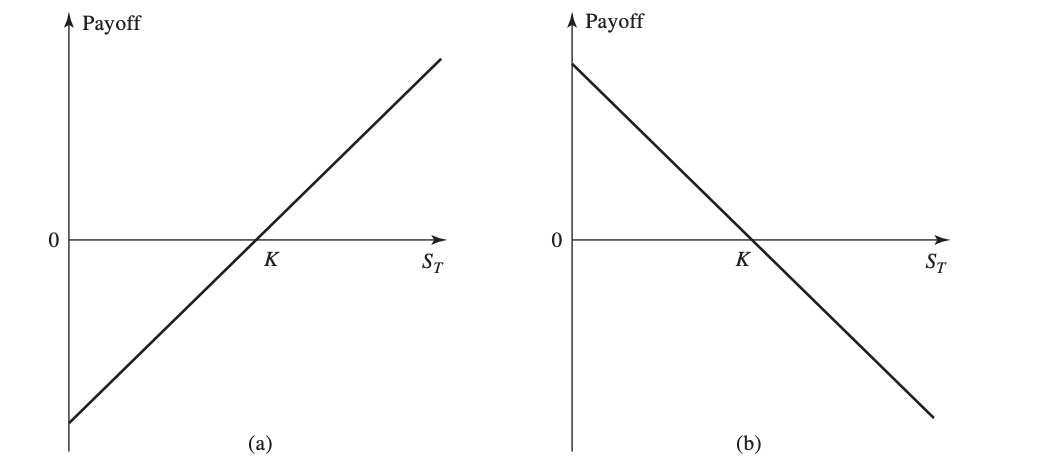
\includegraphics[width=0.8\textwidth]{im4}
    \caption{Guadagni dai contratti forward: (a) posizione lunga, (b) posizione corta.
Prezzo di consegna = K; prezzo dell'asset alla scadenza del contratto = ST.}
    \label{etichetta-univoca2}
\end{figure}

I contratti forward sono utilizzati principalmente per due scopi:

\begin{itemize}
    
\item \textbf{Copertura} (Hedging): le imprese adottano contratti forward per ridurre il rischio associato alle possibili fluttuazioni dei prezzi degli asset, all'interno del mercato di riferimento. Tramite la loro stipula, possono bloccare un prezzo specifico in anticipo e proteggersi contro le variazioni future dei prezzi, così da permettere alle aziende di pianificare le operazioni in modo più efficace, sapendo esattamente quanto pagheranno o riceveranno per il bene sottostante alla scadenza del contratto.

\item \textbf{Speculazione}: gli investitori possono utilizzare i contratti forward per speculare sui movimenti futuri dei prezzi degli asset. Se prevedono che il prezzo di un bene aumenterà in futuro, per esempio, possono acquistare un contratto forward per beneficiare del prezzo concordato anche se il prezzo di mercato sarà superiore alla scadenza del contratto. Al contrario, se si prevede una diminuzione dei prezzi, potrebbero vendere un contratto forward per acquistare il bene al prezzo pattuito, anche se il prezzo di mercato risulterà essere inferiore a scadenza.

\end{itemize}

Tuttavia, è importante sottolineare che queste soluzioni presentano anche alcuni rischi, come il rischio di credito (il rischio che una delle parti non adempia agli obblighi del contratto) e il rischio di liquidità (il rischio di non riuscire a trovare una controparte disposta a concludere l'accordo), che possono minare la stabilità finanziaria delle parti coinvolte, con problematiche annesse, e possono influenzare negativamente l'integrità e l'efficienza del mercato.

\subsection{Contratti Future}

I contratti futures sono strumenti finanziari derivati negoziati su mercati regolamentati, noti come borse merci o mercati dei futures. Questi contratti rappresentano accordi standardizzati tra due parti, in cui si impegnano a comprare o vendere un bene sottostante (come commodities, valute, indici azionari o obbligazioni) a un prezzo predeterminato in una data futura prestabilita da contratto tra le parti.

La caratteristica distintiva dei contratti futures risiede nella loro standardizzazione, che riguarda aspetti cruciali quali, per esempio, la quantità del bene sottostante, la data di scadenza del contratto (consegna) e il prezzo di negoziazione. Questi parametri sono fissati in anticipo dalle autorità regolatorie o dagli organismi di mercato, eliminando la necessità di negoziare dettagli personalizzati tra le parti coinvolte. Grazie a questa uniformità, i contratti futures possono essere facilmente scambiati tra gli operatori di mercato senza la necessità di accordi personalizzati, garantendo maggiore liquidità e accessibilità.

La data di scadenza, in particolare, rappresenta il momento in cui il contratto giunge a termine e la consegna del bene sottostante deve essere obbligatoriamente effettuata. Tuttavia, è essenziale notare che la maggior parte degli operatori di mercato effettua operazioni di "chiusura" prima della scadenza, annullando la necessità di effettuare la consegna fisica del bene. In questo modo, evitano problemi economici e logistici associati alla gestione fisica delle merci e possono concentrarsi unicamente sulla speculazione o sulla copertura delle fluttuazioni dei prezzi, generando profitti più consistenti.

I contratti futures sono utilizzati per una vasta gamma di scopi. Gli investitori e le imprese possono impiegarli per coprirsi dai rischi derivanti da fluttuazioni dei prezzi degli asset sottostanti, come ad esempio potrebbe effettuare un produttore che può utilizzare un contratto future per bloccare un prezzo garantito di vendita di un prodotto e proteggersi da potenziali diminuzioni future dei prezzi contemporaneamente. D'altra parte, uno stesso investitore potrebbe utilizzare un contratto future per speculare sulla direzione futura dei prezzi, cercando di ottenere profitti dalle variazioni del valore dell'asset sottostante nella finestra temporale prevista dall'accordo.


\subsection{Contratti di Opzione}

I contratti di opzione rappresentano accordi tra due parti, noti solitamente come titolare dell'opzione e scrittore dell'opzione, che conferiscono al titolare il diritto, ma non l'obbligo, di comprare (opzione di acquisto o "call") o vendere (opzione di vendita o "put") un bene sottostante (come azioni, valute, indici o commodities) a un prezzo predeterminato, noto come "prezzo di esercizio" o "strike price," in una data futura prestabilita.

A differenza dei contratti futures o forward, in cui le parti si impegnano a comprare o vendere il bene sottostante, i contratti di opzioni restituiscono, al titolare, il diritto di decidere se esercitare o meno l'opzione stessa. Ciò significa che quest'ultimo può trarre vantaggio dall'operazione solo se è conveniente farlo, in base alle condizioni di mercato al momento della scadenza (o all'interno dell'intervallo di tempo stabilito da contratto), decidendo, nel caso ci sia un ritorno economico, di esercitare il proprio diritto di acquisto. D'altro canto, lo scrittore dell'opzione è obbligato a soddisfare gli obblighi dell'opzione se il titolare decide di esercitarla, andando così incontro a possibili perdite finanziarie.

Nello specifico, le opzioni di acquisto (call) offrono al titolare la possibilità di acquistare il bene sottostante al prezzo di esercizio se il prezzo di mercato dell'asset sottostante $S_T$ è superiore allo \textit{strike price} K al momento della scadenza del contratto (o in momenti precedenti alla scadenza, in funzione della tipologia di opzione stipulata), cosi che il titolare possa trarre profitto esercitando l'opzione. Se, al contrario, il prezzo di mercato dell'asset è inferiore al prezzo di esercizio, il titolare può scegliere di non esercitare l'opzione, limitando la sua perdita al premio pagato per l'opzione stessa. 

\begin{equation}
    C = \max (0; S_T - K)
\end{equation}

Le opzioni di vendita (put), d'altra parte, offrono al titolare il diritto di vendere il bene sottostante al prezzo di esercizio K se il prezzo di mercato dell'asset sottostante $S_T$ risulta inferiore al concordato, al momento della scadenza dell'opzione. Così facendo, l'holder può trarre profitto esercitando l'opzione e vendendo il bene a un prezzo superiore rispetto al prezzo di mercato corrente. Se il prezzo di mercato dell'asset è invece superiore al prezzo di esercizio, il titolare può scegliere di non esercitare l'opzione, limitando la sua perdita al premio pagato per l'opzione stessa, così come avviene per le opzioni call.

\begin{equation}
    P = \max ( 0; K - S_T)
\end{equation}

\begin{figure}
     [ht]
    \centering
    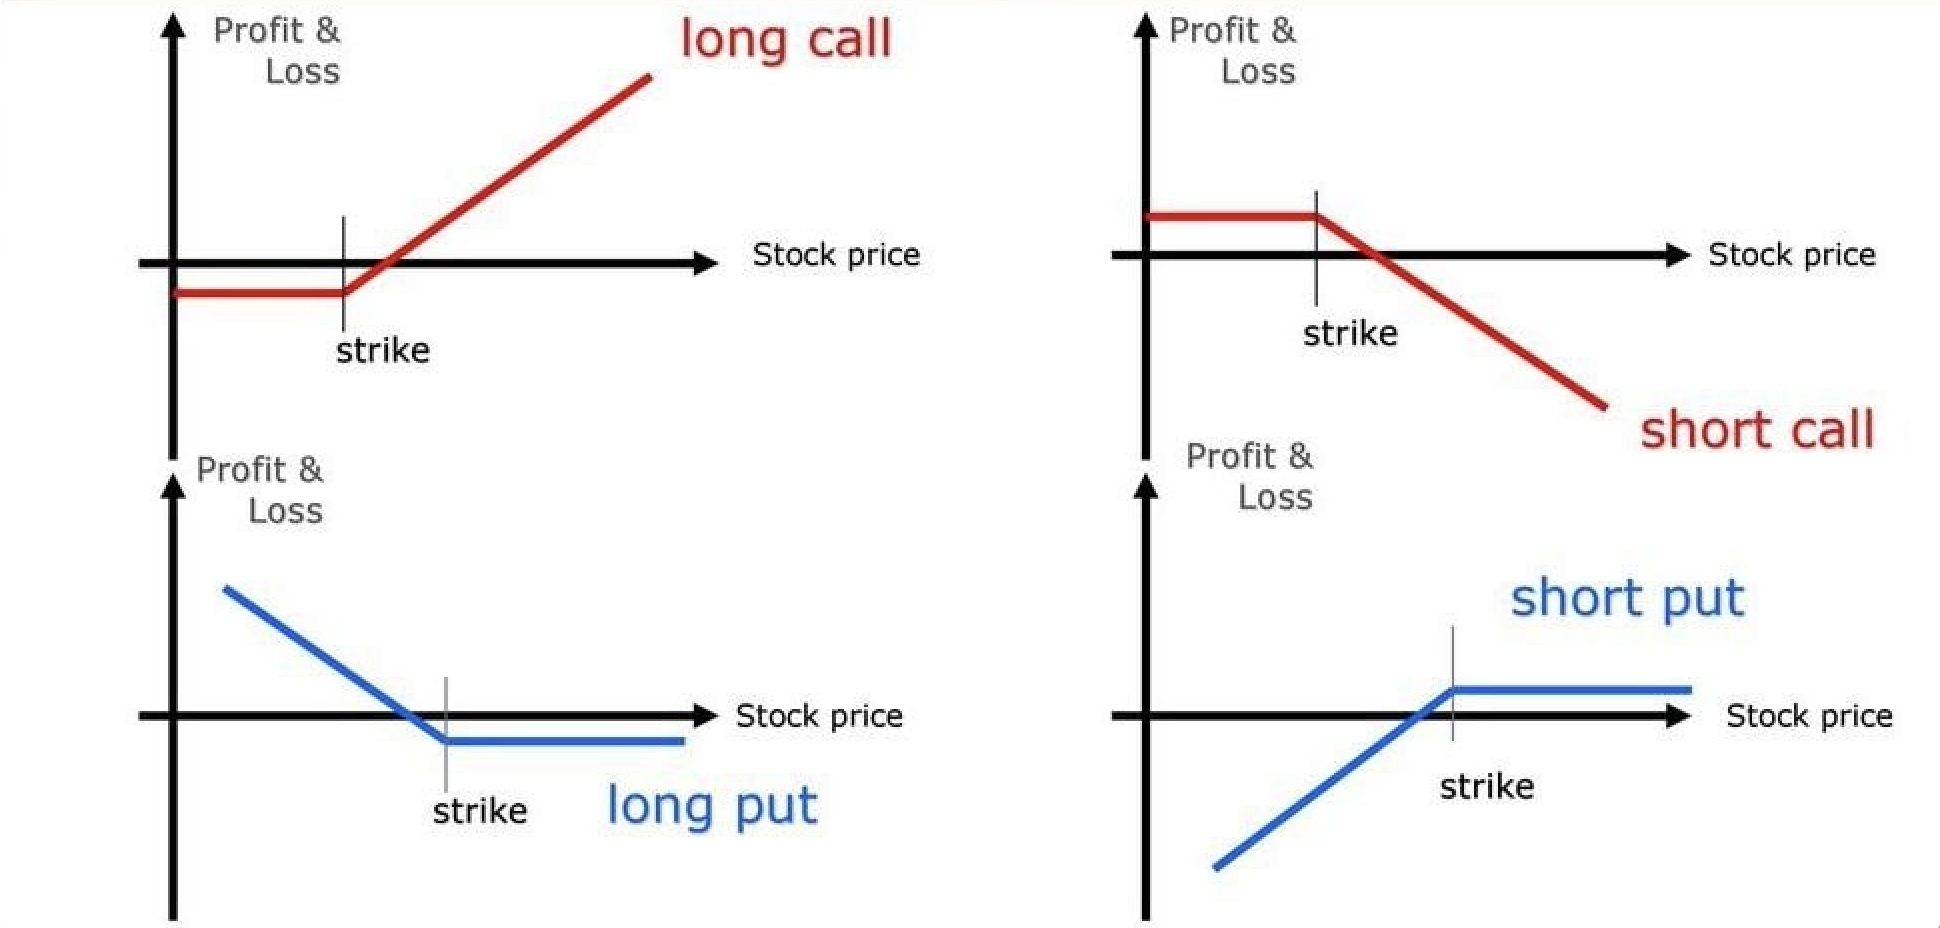
\includegraphics[width=1.0\textwidth]{im5}
    \caption{Posizione lunga e posizione corta delle opzioni Call e opzioni Put }
    \label{fig:enter-label1}
\end{figure}


Le opzioni offrono quindi agli investitori diverse opportunità di speculazione o copertura. Gli investitori possono utilizzarle per sfruttare le previsioni di movimenti futuri dei prezzi, ridurre l'esposizione al rischio di mercato o generare reddito attraverso la vendita di opzioni scoperte (naked option\footnote{Si realizza quando il writer (o venditore) non possiede una posizione di segno opposto sull'attività sottostante il contratto di opzione}).


\subsection{Contratti Swap}

Gli swap rappresentano importanti contratti derivati nel mercato over-the-counter, tali per cui sia possibile concordare tra due parti uno scambio di pagamenti in date future, basati su alcune variabili di mercato come tassi di interesse (come il London Interbank Offer Rate, noto come Libor) e tassi di cambio.
Le istituzioni finanziarie, come banche e società, utilizzano comunemente i contratti swap per gestire o ridurre il rischio di esposizione a tassi di interesse variabili o fluttuazioni di valuta, nel corso del tempo. Le parti coinvolte sono spesso denominate "controparte" o "partecipante allo swap".

Una delle principali caratteristiche riguardanti questi particolari strumenti, risiede nella presenza di più finestre di pagamento previste da contratto, mentre, per esempio, i forwards prevedono un unico pagamento, cosi che si possa considerare quest'ultimi come contratti swap base (o semplici).

Le due tipologie principali di contratti sono gli \textit{interest rate swap} e i \textit{currency swap}. L'i\textit{nterest rate swap} più comune è il "plain vanilla", in cui una controparte si impegna a pagare un tasso fisso basato su un capitale nominale all'altra, che paga un tasso di interesse variabile sullo stesso capitale e per lo stesso numero di periodi.

Lo swap in cui un tasso fisso viene scambiato con uno variabile può essere visto come un portafoglio di obbligazioni, il cui valore (Vswap) è dato dalla differenza tra l'obbligazione con tasso fisso (Bfix) e quella con tasso variabile (Bfl):

\begin{equation}
    V_{\text{swap}} = B_{\text{fix}} - B_{\text{fl}}
\end{equation}


Gli \textit{interest rate swap} possono essere negoziati sotto diverse forme, come \textit{payer swap}, in cui l'acquirente paga i tassi fissi e riceve i tassi variabili, e \textit{receiver swap}, in cui l'acquirente riceve i tassi fissi e paga i tassi variabili.

I \textit{currency swap} funzionano sulla medesima logica di base, ma coinvolgono lo scambio di capitali in diverse valute.

Altri tipi di swap includono i \textit{commodity swap}, che possono essere considerati come una serie di contratti forward, con diverse scadenze ma con lo stesso prezzo di consegna, e il cui sottostante è una merce. 



\chapter{I Derivati energetici}



Il mercato energetico è uno degli ambiti più dinamici e complessi dell'economia globale, influenzato da una vasta gamma di fattori geopolitici, tecnologici e ambientali. Le commodities energetiche, tra cui petrolio, gas naturale, elettricità e carbone, rivestono un ruolo fondamentale nel soddisfare la crescente domanda energetica mondiale della società odierna. Tuttavia, il settore energetico è notoriamente volatile e soggetto a fluttuazioni dei prezzi, che possono essere innescate da una serie di eventi politici o cambiamenti nei fattori di domanda e offerta. Questa instabilità dei prezzi pone le imprese energetiche di fronte a sfide significative nella gestione dei rischi finanziari e operativi.

Per farne fronte, le società energetiche si affidano sempre più ai derivati energetici, che rappresentano strumenti finanziari essenziali per mitigare il rischio di esposizione al mercato delle commodities. Questi strumenti offrono un'ampia gamma di opzioni per le imprese, consentendo loro di proteggersi dalle fluttuazioni dei prezzi, garantire la stabilità finanziaria e prendere decisioni strategiche informate. 

In questo capitolo ci addentriamo più nello specifico, nel mondo delle materie prime energetiche, descrivendo, nei paragrafi successivi, i principali mercati in cui è possibile ritrovare lo scambio di titoli derivati, le commodities di base su cui verte il payoff del contratto e infine il funzionamento delle tipologie contrattuali intraviste nel capitolo precedente ma associate al mercato energetico.


\section{Definizione e caratteristiche dei mercati energetici}


La complessità del commercio energetico deriva principalmente dalle caratteristiche fisiche delle materie prime e dal procedimento di smistamento di quest'ultima nelle aree geografiche di interesse. In particolar modo, l'energia è una risorsa complessa da trasportare e immagazzinare, contrariamente ad altre materie prime. Di fatti, gran parte degli scambi energetici avviene attraverso la consegna fisica della merce. Quando la consegna o la ricezione di un prodotto è parte integrante dello scambio, si parla di "scambio fisico". Al contrario, quando un'operazione comporta solo il trasferimento di denaro contante senza effettiva consegna fisica del bene, si parla di "commercio finanziario". Il trading fisico è caratterizzato da una maggiore complessità rispetto al trading finanziario, ma offre anche maggiori possibilità di gratificazione finanziaria.

La regolamentazione dei mercati energetici fisici è essenziale per gestire le sfide legate alla logistica e alla disponibilità delle risorse energetiche.
I principali prodotti energetici, come l'elettricità e il calore, presentano una sfida unica poiché non possono essere facilmente immagazzinati, ma devono essere generati in tempo reale in base alla domanda. Inoltre, la trasmissione di energia su lunghe distanze risulta molto spesso complessa da attuare, visti gli elevati costi di trasporto annessi. Pertanto, per soddisfare le esigenze dei consumatori, l'energia e il calore vengono tipicamente generati in prossimità delle aree di consumo.

Come stretta conseguenza, il mercato dell'energia è ulteriormente suddiviso in altre due componenti : un insieme di piccoli mercati locali interessati all'attività odierna (mercati spot\footnote{Una transazione spot comporta un trasferimento di merci sul posto. Un sinonimo di spot è cash, come nel \textit{cash market}.}) e un mercato separato concentrato sulle aspettative future a livello nazionale (mercato forward\footnote{Una transazione a termine comporta un trasferimento di merci in un momento futuro. Ad esempio, un accordo per la consegna del gas naturale nel semestre successivo.}).

A differenza del mercato azionario o obbligazionario, i mercati a pronti e a termine dell'energia non sono strettamente collegati, questo perché è impossibile acquistare elettricità in un determinato momento, immagazzinarla e consegnarla in un secondo momento.
Nel settore dell'energia elettrica, i sistemi di trasmissione, noti come reti elettriche, sono spesso gestiti dai governi locali. Tuttavia, quando un operatore di sistema di trasmissione (TSO) non ha collegamenti con il governo locale, viene denominato Operatore di sistema indipendente (ISO). Un ISO che opera su più stati o regioni è comunemente chiamato operatore di trasmissione regionale (RTO). La maggior parte degli scambi di elettricità avviene attraverso reti elettriche gestite da RTO/ISO, soprattutto nei mercati deregolamentati, in cui è permesso il libero scambio di energia elettrica. È importante notare che le regole e le normative possano variare tra le diverse reti elettriche locali, quindi di per sé, non esiste una vera e proprio regolamentazione universale. Inoltre, anche se alcuni mercati energetici sono deregolamentati, la maggior parte di essi è ancora soggetta a una regolamentazione significativa.

Sotto il profilo del trading, i mercati spot presentano una notevole complessità. Sono soggetti a un vasto insieme di normative locali e vincoli fisici. Tuttavia, i mercati forward risultano essere i più liquidi e ciò potrebbe portare a trascurare i mercati fisici a vantaggio dei mercati finanziari, considerati più semplici da comprendere. Tuttavia, al contrario di come si potrebbe pensare, tale atteggiamento costituirebbe un errore. Infatti, i mercati finanziari contengono una vasta gamma di caratteristiche che risultano inspiegabili se non si possiede una comprensione approfondita dei mercati fisici; d'altro canto, la complessità dei mercati spot fisici costituisce il fondamento stesso del commercio di energia. Ciascuno di questi problemi, preso individualmente, può essere di facile comprensione, ma il loro numero elevato richiede un'attenta considerazione e monitoraggio costante.

L'apertura del mercato dell'energia al libero scambio di elettricità è un concetto relativamente recente. Prima della deregolamentazione, solo le centrali elettriche possedute dai servizi pubblici avevano il diritto di vendere energia sulla rete elettrica. Con la deregolamentazione, questo monopolio è stato eliminato, consentendo a chiunque di costruire e gestire una centrale elettrica e offrire energia in vendita. Nei mercati deregolamentati, i servizi pubblici si sono spostati dalla gestione delle centrali alla gestione delle reti di trasmissione. Attualmente, esistono centrali elettriche di proprietà di commercianti di energia e gestite da società specializzate nel settore. Questi cambiamenti hanno rivoluzionato l'industria energetica, creandone un mercato aperto.
Tra gli attori coinvolti nel mercato vi sono i trader, gli investitori e gli operatori di marketing.
Investire nell'esplorazione o nella costruzione di nuovi impianti di produzione richiede ingenti capitali, spesso raccolti dagli investitori. Il principale obiettivo delle utility locali risulta garantire una fornitura costante di energia ai propri clienti mediante contratti finanziari per l'acquisto di combustibile ed elettricità. Le centrali elettriche, d'altra parte, acquistano il combustibile necessario per produrre elettricità e successivamente la vendono. Le grandi aziende industriali potrebbero desiderare garantire forniture future di energia a prezzi stabili mentre, allo stesso tempo, società finanziarie possono voler speculare sul prezzo dell'energia. Per realizzare queste operazioni, tutte le parti coinvolte possono effettuare transazioni finanziarie \textit{over the counter}, che possono essere condotte direttamente tra due parti o attraverso l'intermediazione di un terzo soggetto. I prodotti energetici sono comunemente scambiati sul New York Mercantile Exchange (NYMEX\footnote{Rappresenta la maggiore borsa per lo scambio dei titoli azionari rappresentativi del mercato delle materie prime, dei metalli preziosi e dei prodotti energetici}) e sull'Intercontinental Exchange (ICE).

\subsection{Tipologie di commodities energetiche:}

Il mercato dell'energia è un complesso sistema costituito da diversi prodotti distinti, riguardanti la produzione e la fornitura di elettricità e calore. Tra questi, i due più significativi sono il gas naturale e l'elettricità. Altri beni secondari presenti nel mercato includono il carbone, le emissioni di carbonio e le fonti di energia alternativa. Il petrolio è anch'esso un prodotto energetico, ma la sua influenza è maggiormente rilevante come fonte di energia per il settore automobilistico, piuttosto che per la generazione di elettricità e calore all'interno delle abitazioni o luoghi di lavoro. Nonostante ciò, l'impatto economico del petrolio è così rilevante che esso gioca un ruolo di primaria importanza in ogni aspetto del commercio energetico mondiale. 


\subsubsection{Petrolio Greggio}

Il petrolio greggio è una delle materie prime più preziose e fondamentali nel mercato. È una miscela di idrocarburi liquidi, con una composizione chimica complessa e variegata. La qualità del petrolio greggio varia in base al suo peso specifico e al contenuto di composti solforati.  
Una volta estratto, viene sottoposto a un processo di raffinazione noto come distillazione, che consente di separare i suoi componenti in diverse frazioni in base alla loro temperatura di ebollizione. Durante la distillazione, il petrolio viene riscaldato e i vapori risultanti vengono raffreddati e condensati in prodotti finiti. 

Alcuni dei prodotti finiti ottenuti dalla raffinazione del petrolio includono:

\begin{itemize}
  \item Benzina per auto (gasoline): Questo è uno dei prodotti più importanti ottenuti dalla raffinazione del petrolio. È un carburante utilizzato principalmente nei motori a combustione interna delle automobili.
  \item Gasolio da riscaldamento (heating oil): Questo prodotto è utilizzato per riscaldare edifici e altre strutture durante i mesi più freddi dell'anno.
  \item Nafta (fuel oil): La nafta è utilizzata come combustibile per applicazioni industriali, come ad esempio nelle centrali termiche.
  \item Cherosene (kerosene): Il cherosene è utilizzato come combustibile per lampade, motori aeronautici e stufe.
\end{itemize}

La raffinazione del petrolio greggio è un processo complesso e tecnologicamente avanzato, che permette di ottenere una vasta gamma di prodotti essenziali per la nostra società, principalmente riguardanti la mobilità. La sua qualità e la sua composizione influenzano direttamente i prezzi dei prodotti finiti, e quindi hanno un impatto significativo sull'economia globale e sulle dinamiche dei mercati energetici. Difatti, il mercato del greggio è il più importante mercato di merci al mondo, con una domanda globale pari a circa 90 milioni di barili al giorno. Da molti anni vengono negoziati sul mercato \textit{over the counter} contratti di fornitura a prezzo fisso con scadenza decennale. Si tratta di \textit{swaps} in cui si scambia il petrolio a prezzo fisso con il petrolio a prezzo variabile.
I punti di riferimento fondamentali per la determinazione dei prezzi del petrolio greggio sono il Brent e il West Texas Intermediate (WTI). Il Brent è un tipo di petrolio estratto dalle acque del mare del Nord, mentre il WTI proviene dalla regione del Texas, negli Stati Uniti. Questi due benchmarks sono ampiamente utilizzati per il trading e il pricing del petrolio greggio.

Nei mercati \textit{over the counter}, i derivati basati su diverse attività finanziarie, come azioni e indici azionari, sono anche ampiamente disponibili per il petrolio come sottostante. Nello specifico, in questo contesto, contratti come \textit{forwards, swaps} e \textit{opzioni} sono ampiamente diffusi e offrono agli investitori strumenti flessibili per gestire il rischio e partecipare alle fluttuazioni dei prezzi del petrolio.
L'attrattiva dei derivati petroliferi risiede nella possibilità di negoziare contratti personalizzati e non standardizzati nei mercati OTC, consentendo alle parti coinvolte di adattare le condizioni alle proprie esigenze specifiche. Questi contratti possono essere liquidati sia per contanti, con pagamenti finanziari delle differenze di prezzo, sia con la consegna fisica effettiva del petrolio.

Attraverso entità come il CME Group e l'Intercontinental Exchange (ICE), i futures e le futures options basati sul petrolio vengono scambiati su base regolare. I futures, essendo contratti standardizzati negoziati in borsa, obbligano le parti a comprare o vendere petrolio a un prezzo e una data futura predefiniti. Alcuni futures prevedono la liquidazione in contanti, mentre altri richiedono la consegna fisica del petrolio.

\subsubsection{Gas naturale}

Il gas naturale è un altro importante combustibile utilizzato in ingenti quantità dalla società odierna. I derivati energetici legati al gas naturale comprendono futures e swap, che consentono alle aziende attive nel settore, di mitigare i rischi associati al valore di mercato di questo particolare elemento. 

In tutto il mondo, l'industria del gas naturale ha attraversato un periodo di deregolamentazione e di eliminazione dei monopoli di Stato, conducendo ad importanti evoluzioni nel mercato di riferimento. Questa trasformazione ha aperto la strada a significativi cambiamenti, in cui le società produttrici e distributrici di gas naturale sono diventate entità separate, con ruoli specifici e indipendenti. Queste imprese hanno ora il compito cruciale di gestire e far fronte alla domanda di mercato giorno per giorno. Deve essere garantita una fornitura adeguata per soddisfare le esigenze dei consumatori, e contemporaneamente, devono essere presi in considerazione i fattori che possono influenzare i prezzi del gas naturale, esponendo cosi le società ad una instabilità finanziaria.
Per la mitigazione dei rischi associati alle fluttuazioni dei prezzi del gas naturale, le società utilizzano derivati energetici come futures e swap, i quali aiutano le aziende a proteggersi dalle fluttuazioni dei prezzi del gas, garantendo una pianificazione finanziaria più efficace e consentendo una gestione più sicura delle operazioni commerciali.

I repentini cambi di prezzo associati al mercato del gas naturale risiedono semplicemente nella varietà del suo utilizzo. Nella fattispecie, è un combustibile ampiamente richiesto sia per il riscaldamento degli edifici che per la produzione di energia elettrica, che a sua volta viene utilizzata per il condizionamento dell'aria e altre applicazioni. A causa di queste diverse esigenze, la domanda varia stagionalmente e segue logiche legate al clima e ai consumi energetici.
In Europa, l'indice di mercato del gas di Amsterdam, tra i più importanti del continente, ha subito una serie di significativi aumenti a partire dalla seconda metà del 2021, superando i 0,3 €/Smc e raggiungendo un picco di 1,20967 €/Smc all'inizio del 2022. Successivamente, a causa degli eventi geopolitici come la guerra in Ucraina e le sanzioni alla Russia, il TTF\footnote{ TTF è l’acronimo di "Title Transfer Facility", ossia il mercato all’ingrosso del gas naturale tra i più grandi d’Europa. Ha sede ad Amsterdam in Olanda (l’indice è anche chiamato in inglese "Dutch TTF gas price") e rappresenta il principale punto di riferimento per i prezzi del gas in Europa e in Italia.} ha avuto un rimbalzo negativo, ma ha poi ripreso a crescere fino a raggiungere quota 2,482083 €/Smc nel settembre 2022.
Tuttavia, il mese di ottobre 2022 ha segnato una prima inversione di tendenza, con il TTF che è sceso a 2,166775 €/Smc, e questo calo è continuato nei mesi successivi con valori di 1,417546 €/Smc a novembre 2022 e una media di 1,269805 €/Smc a dicembre 2022.
Il 2023 è iniziato con un netto calo del prezzo del TTF, con una quotazione media di 0,576 €/Smc a febbraio, arrivando a 0,339 €/Smc a maggio e 0,342 €/Smc a giugno. Sebbene ci sia stato un calo rispetto ai picchi raggiunti nel 2022, l'indice rimane comunque nettamente superiore ai valori pre-crisi del 2021.
Per un ritorno alla normalità è necessario un ulteriore calo dell’indice, che continuerà a influenzare l'intero mercato energetico, soprattutto nel breve periodo. Il grafico riporta l’andamento dell’indice nel corso degli ultimi 24 mesi.
$$
$$
\begin{figure}
     [ht]
    \centering
    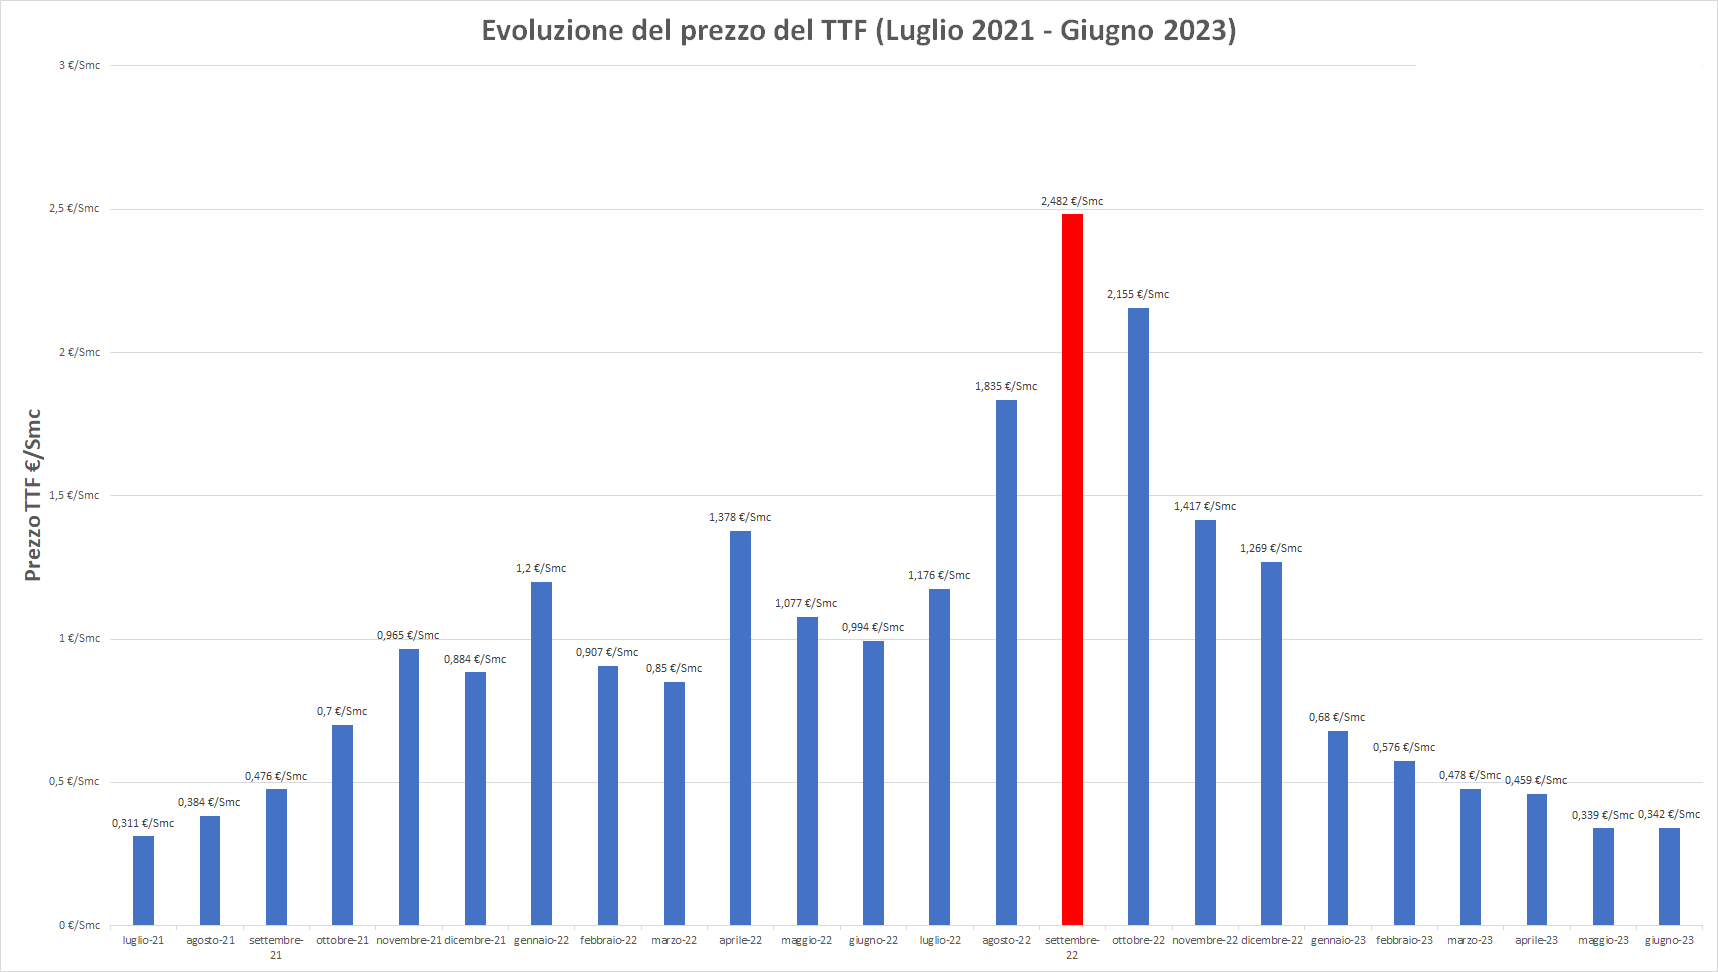
\includegraphics[width=1.0\textwidth]{im3}
    \caption{Evoluzione del prezzo del TTF Luglio 2021 - Giugno 2023 
            (Fonte: European Gas Spot Index)}
    \label{fig:enter-label2}
\end{figure}
$$
$$

\subsubsection{Carbone}

Il carbone è un combustibile idrocarburico solido facilmente disponibile in tutto il mondo. È facile da immagazzinare e relativamente poco costoso da produrre rispetto alla quantità di energia elettrica che può generare, tale per cui è possibile intravederlo come il carburante perfetto. Sfortunatamente, è una delle principali fonti di emissioni di carbonio (CO2) e zolfo (SO2), una delle cause principali dell'inquinamento atmosferico registrato nel corso della storia. Difatti, quando parliamo di carbonio e del suo utilizzo, spesso ci troviamo di fronte a desideri contrastanti: da un lato, l'aspirazione a un'energia elettrica economica e accessibile e, dall'altro, la necessità di ridurre l'inquinamento causato dalle emissioni di carbonio. Questa contraddizione ha portato a sforzi globali bloccati sulla questione della generazione a carbone. Molti paesi desiderano continuare a utilizzare centrali elettriche a carbone per ragioni di costo, ma allo stesso tempo sperano che altri paesi riducano o eliminino il suo utilizzo per mitigare l'inquinamento ambientale.

I derivati energetici legati al carbone sono principalmente swap e contratti a termine, utilizzati per coprire il rischio di fluttuazioni dei prezzi del carbone, ma non sono notoriamente preferiti per i concetti descritti precedentemente.

\subsubsection{Elettricità}

L'elettricità è una materia prima unica tra le commodities energetiche poiché non può essere immagazzinata. Ed è proprio da questa sua caratteristica che si creano sfide uniche per la gestione e copertura del rischio. I derivati energetici legati all'elettricità includono futures, forwards e opzioni, che consentono alle aziende di gestire il rischio di fluttuazioni dei prezzi dell'energia elettrica.
La massima fornitura di elettricità di cui può usufruire un qualsiasi territorio, in un dato istante, è determinata dalla massima capacità di tutti gli impianti che generano risorse elettriche nella regione corrispondente al territorio osservato. 
Per esempio, negli Stati Uniti ci sono 140 regioni note come "aree di controllo" (control areas). Qualora risultino eccedenze di elettricità nell'area di controllo specifica, il sistema prevede la possibilità di vendere ad ulteriori aree la merce non utilizzata. Sulla base di queste eccedenze si origina il mercato all'ingrosso di energia elettrica, in cui tali aree sono in grado di vendere tanta più energia quanto è maggiore la capacità di trasmissione delle linee che collegano le diverse regioni.

Tra i maggiori utilizzatori di elettricità figurano i sistemi di condizionamento dell'aria. Come ci si può aspettare, soprattutto negli ultimi anni, la domanda estiva ha subito notevoli rialzi, causati soprattutto da violente ondate di calore, comportando aumenti del prezzo \textit{spot} dell'ordine del 1.000\%, per brevi periodi.

\begin{figure}
    \centering
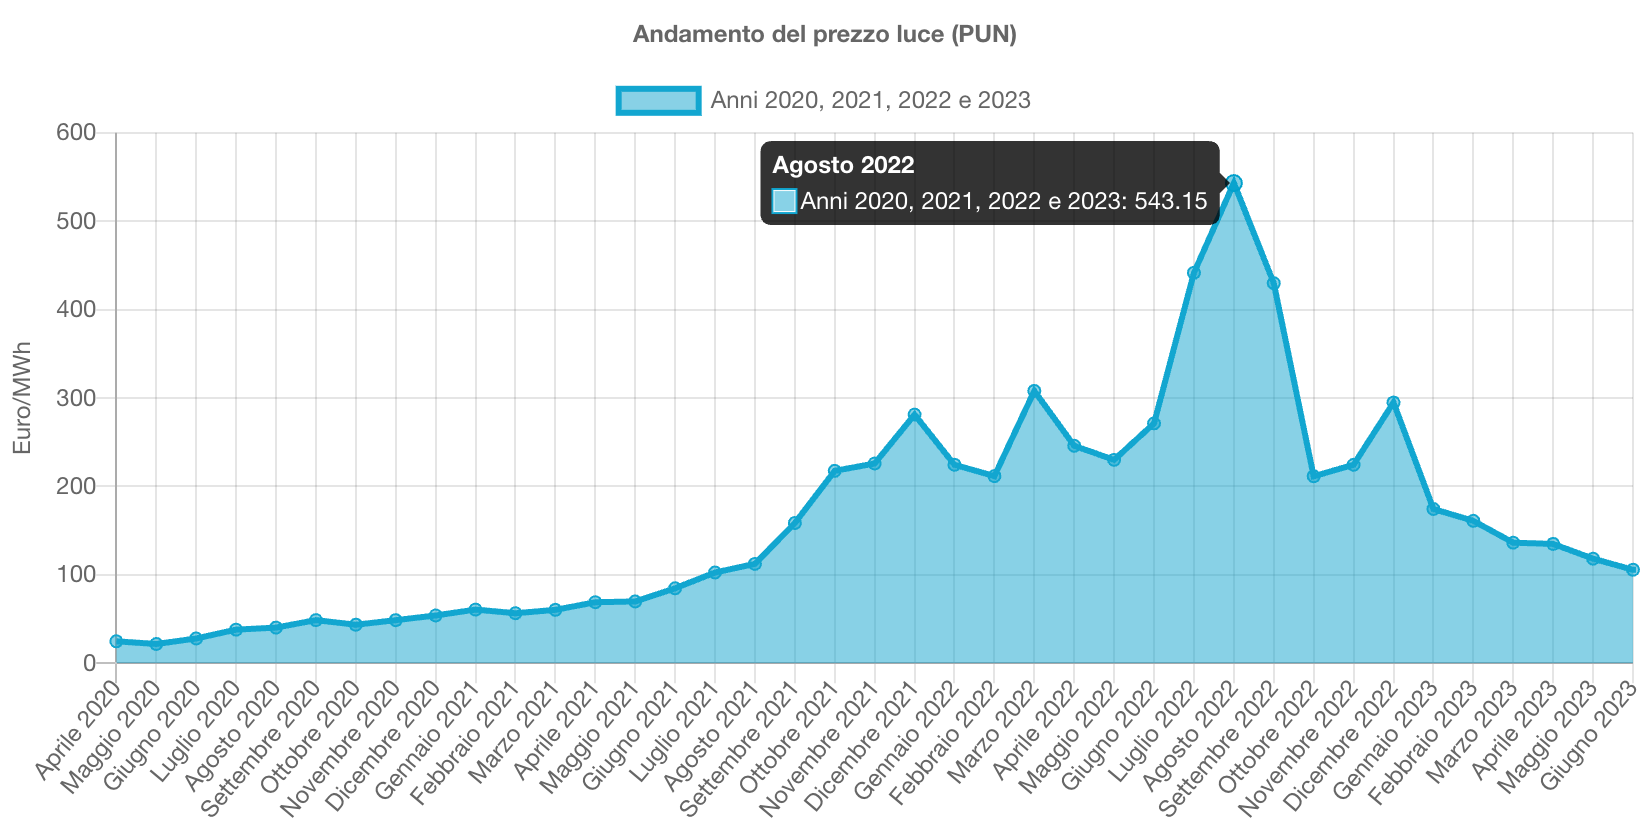
\includegraphics[width=0.8\textwidth]{im1}
\caption{Andamento del prezzo luce (PUN) Aprile 2020 - Giugno 2023 (Fonte: GME)}
    \label{fig:enter-labelgas}
\end{figure}

Analogamente al gas naturale, l'industria dell'energia elettrica ha attraversato un periodo di deregolamentazioni e di eliminazione dei monopoli di Stato, con conseguenziale sviluppo di un mercato di derivati sull'elettricità. Al CME Group viene ora trattato un \textit{futures} sul prezzo dell'elettricità e sul mercato \textit{over the counter} si negoziano attivamente \textit{forwards, swaps} e opzioni. Normalmente, i contratti, che siano negoziati in borsa o nel mercato OTC, prevedono la fornitura per un mese di una determinata quantità di megawatt/ora in una particolare area geografica, ad un prezzo naturalmente prefissato.

L'esercizio delle opzioni sull'energia elettrica può essere giornaliero o mensile. Nel primo caso, per esempio, il portatore dell'opzione ha il diritto di ricevere, in un qualsiasi giorno del mese, una certa quantità di energia al prezzo d'esercizio prefissato. Nel secondo caso invece, la decisione inerente la quantità di energia elettrica richiesta per l'intero mese al prezzo prefissato va presa all'inizio del mese.

Una tipologia di contratto molto interessante che viene negoziata sia nei mercati elettrici, sia in quelli del gas naturale, è noto come "opzione di variazione (\textit{swing option}) o "opzione 'prendi e paga'" (\textit{take-and-pay option}). Nello specifico, l'opzione di variazione consente all'acquirente di adattare la quantità di energia o gas richiesta in base alle variazioni della domanda o alle esigenze operative. Ciò significa che l'acquirente ha il diritto, ma non l'obbligo, di acquistare o fornire una quantità variabile di energia o gas a un prezzo concordato durante un periodo di tempo specificato. Questa flessibilità è particolarmente utile in scenari in cui la domanda può variare notevolmente a causa di condizioni meteorologiche, eventi imprevisti o esigenze operative. Ad esempio, un'azienda energetica potrebbe acquistare un'opzione di variazione per l'approvvigionamento di energia elettrica durante l'inverno, quando la domanda si aspetta essere influenzata dal clima rigido e dall'elevata richiesta di riscaldamento residenziale e industriale. In questo caso, l'azienda può scegliere di acquistare e pagare solo per la quantità di energia effettivamente necessaria in base alla domanda effettiva, evitando di dover pagare per eccessi di energia non utilizzata.
Il medesimo esempio è applicabile anche al mercato del gas naturale. Un'azienda che utilizza gas come combustibile per le sue operazioni potrebbe stipulare un'opzione di variazione per adattare la quantità richiesta in base alla produzione, alla domanda e alle fluttuazioni dei prezzi.

L'opzione di variazione può quindi offrire benefici sia agli acquirenti che ai fornitori in entrambi i mercati. In particolar modo, per gli acquirenti offre maggiore flessibilità nella gestione della domanda e può ridurre i rischi associati all'incertezza insita nel mercato di riferimento; per i fornitori invece, può aiutare a ottimizzare l'utilizzo delle risorse e a soddisfare meglio le aspettative dei clienti senza dover sostenere costi eccessivi per l'energia o il gas in eccesso.


\section{Forwards, futures and swaps energetici:}


I contratti forward, future e swap sono strumenti di copertura del rischio, ma differiscono dalle opzioni poiché non presentano "optionality". Questo significa che quando si utilizzano questi strumenti, le parti coinvolte sono vincolate a eseguire l'accordo in modo definitivo alla scadenza, indipendentemente dalle condizioni di mercato. Al contrario, con le opzioni, come abbiamo accennato precedentemente, il detentore ha la flessibilità di decidere se esercitare o meno il diritto di acquistare o vendere l'asset in base alla situazione di mercato al momento della scadenza. Inoltre, essi costituiscono la tipologia di derivati più liquidi che esista e sono più facili da utilizzare e valutare rispetto alle opzioni. Nel paragrafo successivo, andremo ad analizzare le principali caratteristiche associate a queste tipologie di coperture, connesse al mondo energetico.

\subsection{Forward sull'energia}

Essendo accordi privati tra due parti, i contratti forward vengono negoziati nel mercato over-the-counter (OTC). 

Nel caso delle materie prime, essi consistono in accordi bilaterali per acquistare o vendere una determinata quantità di una materia prima (petrolio, gas, elettricità) in una data di consegna fissa, a un prezzo contrattuale predeterminato, con pagamento solitamente a scadenza.

Un esempio semplice di contratto forward può riguardare una transazione su una qualsiasi materia prima, come il petrolio greggio, gas naturale ecc. In particolar modo, immaginiamo che un produttore di petrolio e una raffineria vogliano evitare l'incertezza legata alle fluttuazioni del prezzo sul mercato nel prossimo anno. Entrambe le parti hanno il diritto di stipulare un contratto forward in cui si impegneranno a vendere e comprare una determinata quantità di petrolio greggio a un prezzo concordato, ad esempio \$70 al barile, tra un anno dalla data dell'accordo, fissando così un prezzo invariante. Questo accordo è vincolante e le parti sono obbligate a rispettarlo, indipendentemente da quale sia il prezzo di mercato del petrolio al momento della scadenza del contratto. Se alla scadenza il prezzo di mercato è superiore al prezzo di forward, il produttore venderà il petrolio alla raffineria a un prezzo inferiore rispetto al prezzo di mercato, beneficiando così la raffineria. Viceversa, se il prezzo di mercato è inferiore al prezzo di forward, la raffineria dovrà comunque acquistare il petrolio al prezzo pattuito, subendo quindi una perdita rispetto al prezzo di mercato corrente.

Cosi come nel caso generico, i principali utilizzi dei forward sull'energia sono principalmente tre: copertura dell'obbligo di consegna o acquisto di una materia prima in una data futura; assicurarsi un profitto dalla produzione di una materia prima; speculare sulle fluttuazioni dei prezzi delle materie prime quando manca un mercato futuro liquido (Burger, 2007).

Come citato precedentemente, all'interno del mercato dell'elettricità, i contratti forward costituiscono la maggioranza degli strumenti utilizzati per la gestione del rischio.  Immaginiamo una complessa struttura energetica, influenzata da elevati fattori casuali che possono portare a significative variazioni nei prezzi dell'elettricità. Per mitigare i rischi associati a tali fluttuazioni, è essenziale trovare un insieme di contratti che siano dipendenti dagli stessi n fattori. Questo insieme di contratti rappresenta una strategia di copertura completa, in grado di bilanciare e ridurre l'esposizione ai rischi del mercato dell'elettricità. 

La scelta oculata di utilizzo di questa tipologia di contratti è fondamentale per proteggere un'azienda, una \textit{utility} o un investitore dai cambiamenti improvvisi e sfavorevoli nei prezzi dell'elettricità; inoltre, grazie alla loro natura personalizzabile e flessibile, i contratti forward possono essere adattati alle specifiche esigenze e alle particolari dinamiche del mercato dell'energia elettrica.

La capacità di trovare un insieme di contratti forward correlati agli stessi fattori casuali è di vitale importanza poiché consente di mitigare il rischio di esposizione e di conseguenza proteggere il valore degli investimenti. Senza una strategia adeguata di copertura, gli operatori potrebbero trovarsi esposti a fluttuazioni di mercato impreviste, che possono portare a perdite finanziarie significative.


\subsection{Futures sull'energia}

I futures sull'energia sono quasi equivalenti ai forward, ma presentano alcuni vantaggi, legati principalmente alla eliminazione del rischio di credito e alla riduzione sostanziale dei costi di transizione previsti, unicamente derivanti dalla standardizzazione del contratto. Un ulteriore elemento interessante deriva dalla possibilità di stimare il valore dei contratti forward attraverso i loro prezzi. Inoltre, la negoziazione giornaliera consente una valutazione facile e frequente del mercato rispetto a forward e swap.

Gli elementi principali dei futures sulla materia prima includono: volume, prezzo, luogo di consegna, periodo di consegna, ultima giornata di negoziazione o data di liquidazione (Eydeland A. e K. Wolyniec, 2003). Il mercato di riferimento in cui vengono negoziati i futures è il NYMEX, ma non solo. Esistono ulteriori borse valori alle quali lo scambio di futures si presta, come la COMEX, uno dei mercati principali in termini di materie prime, o nel caso italiano, sul mercato IDEM (Italian Derivatives Market), attivo dal 1994.

È possibile utilizzare questi strumenti come mera copertura del rischio legato alle fluttuazioni dei prezzi associate alle principali commodities energetiche (petrolio greggio, gas naturale, elettricità ecc.).

Un esempio interessante è fornito da Eydeland e Wolyniec (2003), che immaginano un'impresa A impegnata a fornire energia ai propri clienti durante l'estate, quando i prezzi si suppongono siano elevati, a causa del maggior consumo di elettricità dovuto, nella maggior parte dei casi, ad un utilizzo elevato degli impianti di raffreddamento presenti nelle abitazioni. Il rischio è rappresentato dalla volatilità dei prezzi delle materie prime e la soluzione potrebbe essere quella di fissare i prezzi estivi il prima possibile, in modo tale da scongiurare possibili perdite in futuro. In effetti,  l'impresa A potrebbe decide di negoziare con un'azienda di trading energetico un prezzo fisso inerente alla fornitura di energia per un mese. Verrebbe quindi firmato un future sull'energia, ovvero una delle parti fornirà per un mese una fornitura di energia contrattuale all'altra, impegnata a pagare una somma fissa di denaro. In questo modo, il fornitore di energia previene il rischio di volatilità dei prezzi durante l'estate e scongiura qualsiasi ripercussione finanziaria. 

Questo semplice esempio è fornito per illustrare l'utilità dei futures sull'energia in un contesto altamente volatile come il mercato elettrico. Qui, le fluttuazioni dei prezzi sono molto comuni, soprattutto dal 2020 ad oggi, a causa di eventi esterni come l'innalzamento delle temperature. Il rischio non riguarda solo l'impresa A ma coinvolge anche l'altra azienda, che si trova obbligata a fornire energia in un periodo in cui il prezzo spot\footnote{Il prezzo a pronti (o prezzo spot) è il prezzo che l'acquirente deve corrispondere al venditore per acquistare un bene o un'attività finanziaria la cui consegna è immediata, ossia contestuale alla stipula del contratto di compravendita.} è superiore a quello contrattualmente fissato.

L'unico modo per mantenere la redditività per l'azienda di trading è sottoscrivere una copertura dinamica con futures nei mesi precedenti alla stipula del contratto, sfruttando l'andamento al rialzo e al ribasso dei prezzi e accumulando un margine positivo consistente. Questo permette di fornire energia contrattualmente fissata nel mese specificato alla controparte, senza subire perdite indesiderate.


Fondamentale è quindi per le imprese, operanti in questi settori, implementare una adeguata copertura strategica, che vada, attraverso l'utilizzo di contratti forward o contratti futures, a salvaguardare il prezzo della materia prima energetica scambiata, in modo tale da evitare possibili ripercussioni sul proprio assetto finanziario.  


\subsection{Swap sull'energia}

Gli swap energetici non differiscono di molto rispetto ai contratti forward intravisti nel paragrafo precedente. Infatti è possibile considerare quest'ultimi come "swap uniperiodali", essendo contratti di durata medio-breve termine rispetto invece ai contratti swap che presentano scadenze a lungo termine.
Sono negoziati nei mercati regolamentati OTC, presentano le principali caratteristiche dei contratti derivati come flessibilità, versatilità, personalizzazione e copertura del rischio. Il loro funzionamento prevede solitamente il pagamento di una somma fissa (definita durante la stipula del contratto) erogato a favore di una controparte, mentre a quest'ultima è richiesto un pagamento periodico dipendente dal valore registrato di uno specifico indice variabile scelto, come per esempio il prezzo spot del petrolio greggio o del gas naturale.
Nei mercati OTC energetici esistono diverse tipologie di contratti swap, capaci di garantire versatilità e non rigidità, a copertura dei rischi connessi alla materia prima utilizzata, come: 

\begin{itemize}
    \item \textbf{Plain Swap}: è il contratto swap di base che prevede uno scambio di flussi di cassa o materie prime, dove una delle parti paga un prezzo fisso in una sequenza di pagamenti. Un'azienda può utilizzare gli swap per proteggersi dalle fluttuazioni al rialzo dei prezzi: ad esempio, può pagare un prezzo prestabilito (prezzo dello swap) e ricevere in cambio una determinata quantità di materia prima, anche se i prezzi di mercato superano il prezzo dello swap. In questo modo, quando i prezzi sono elevati, riceve flussi di cassa aggiuntivi, ma non può sfruttare le fluttuazioni al ribasso dei prezzi.
    \item \textbf{Interest Rate Swap} (IRS): tipologia di swap basata sulla gestione del rischio connessa ad un tasso di interesse associato a prestiti e finanziamenti, utilizzati per investire nel settore energetico. Nello specifico, le parti coinvolte scambiano flussi di cassa basati su tassi di interesse, sia fissi che variabili, così da stabilizzare il più possibile i costi connessi ai finanziamenti e, contemporaneamente, ridurre il rischio connesso a possibili rialzi dei tassi.
    \item \textbf{Currency Swap}: contratti che gestiscono il rischio valutario associato a transazioni internazionali, in ambito energetico. In particolar modo, le parti soggette alla stipula del contratto, si impegnano a scambiarsi flussi di cassa (in valute differenti), proteggendosi dalle fluttuazioni che possono registrarsi sui tassi di cambio, garantendo stabilità finanziaria.
    \item \textbf{Load Swap} (Swing swap): equivalenti ai classici contratti swap energetici, con l'unica differenza che, in questo caso, l'oggetto in interesse del contratto non è il valore della materia prima scelta, bensì la quantità di energia richiesta o fornita. In altre parole, ci si assicura contro il rischio associato alle fluttuazioni nella domanda e offerta di energia, nel periodo di interesse.     
\end{itemize}

Queste sono solo alcune delle tipologie di swap energetiche presenti sul mercato. Esistono ulteriori contratti simili ai casi precedenti, ma che differiscono unicamente dall'oggetto di interesse sul quale grava il rischio, come, per esempio, i \textbf{Weather Swap}, basati sul rischio climatico o i \textbf{Emission Swap} collegati ai rischi di emissione di CO2.



\section{Opzioni sull'energia}


Le tipologie di opzioni negoziate nel mercato energetico differiscono per due caratteristiche principali: durata e materia prima. Nello specifico, in funzione del mercato di riferimento, si possono stipulare opzioni fisiche annuali, trimestrali e mensili o opzioni giornaliere, opzioni orarie e opzioni esotiche\footnote{La categoria delle opzioni esotiche fa riferimento a tutti i contratti di opzione in cui il calcolo del payoff presenta elementi di novità rispetto alle opzioni plain vanilla. Questi contratti vengono negoziati OTC (over the counter) proprio a causa della mancanza di standardizzazione degli elementi contrattuali (Borsa Italiana).}(come gli \textit{spread option}). Un ulteriore tipologia negoziata nei mercati energetici è l'opzione cash, un contratto a valenza giornaliera, basato su un prezzo di esercizio fisso o variabile, scelto all'inizio di ogni mese (ad esempio, l'indice giornaliero del gas).
 
 Le opzioni \textbf{plain-vanilla}, che rappresentano la tipologia base di opzioni Call e opzioni Put, possono riguardare una qualsiasi \textit{commodities} energetica scelta come attività sottostante (gas naturale, elettricità, ecc.). Ad esempio, chi possiede un opzione Call energetica ha il diritto, ma non dovere, di richiedere alla controparte (ovvero chi vende l'opzione) di consegnare una determinata quantità di energia, prevista da contratto, in un mese specifico. Viceversa, chi detiene un'opzione Put energetica ha il diritto, ma non l'obbligo, di richiedere alla controparte di acquistare una determinata quantità di energia, prevista dal contratto, in un mese specifico. Naturalmente, entrambe le tipologie di opzione offrono la possibilità al titolare di decidere se esercitare o meno i diritti previsti da contratto, in funzione dell'andamento dell'attività sottostante nel periodo di copertura. Il venditore dell'opzione, d'altra parte, ha l'obbligo di sottostare al volere della controparte, qualora quest'ultimo decida di esercitare l'opzione.  

La principale problematica connessa alla negoziazione di contratti di 
opzione nei mercati energetici riguarda l'impossibilità di negoziare il prezzo spot. Infatti, a differenza di altri mercati in cui è possibile negoziare attivamente il prezzo spot dell'attività sottostante, nei mercati energetici l'energia rappresenta un bene fisico che deve obbligatoriamente essere prodotto, trasportato e consumato all'istante, data l'impossibilità o la quasi-impossibilità di immagazzinare in grandi quantità queste materie prime e, quindi, di acquistarle e rivenderle in giorni differenti. Da tale differenza si collega l'inattuabilità di negoziazione, essendo il prezzo influenzato costantemente da una serie di fattori, definibili "immediati", come la domanda e l'offerta in tempo reale, le condizioni climatiche, eventi geopolitici ed ulteriori eventi imprevisti. Da tale imprevedibilità deriva l'impossibilità di definire un valore fisso nei contratti di opzione.


Una possibile soluzione risulta negoziare questi strumenti sulla base dei prezzi di riferimento derivati, come i prezzi dei future o di altri strumenti correlati al mercato energetico.


Solitamente le opzioni vengono utilizzate unicamente quando nessun altro strumento finanziario si presta alla copertura del rischio. Una comune applicazione è quella di coprirsi in funzione di un aumento straordinario del prezzo spot dell'energia: "un'opzione viene utilizzata come assicurazione contro eventi straordinari" (Eydeland e Wolyniec, 2003), eventi con una bassa probabilità di accadere ma che possono produrre effetti devastanti, come le recenti ondate di calore registrate nella penisola italiana nel corso della stagione estiva. 


\chapter{Modellizzazione dei prezzi per la valutazione dei derivati energetici}

Il fine di questo capitolo è di individuare alcuni modelli in grado di descrivere in modo accurato il comportamento del prezzo a pronti e di fornire il miglior supporto possibile per le operazioni di determinazione dei prezzi dei derivati energetici. Alla luce dell'importanza e della delicatezza associata alla gestione dei rischi operativi e finanziari nell'assicurare il regolare funzionamento dell'impresa, è essenziale riconoscere i processi sottostanti che meglio riflettono la realtà dell'attività.
Si sottolinea che tale intento non mira a una previsione dei prezzi. Se così fosse, ossia se i prezzi futuri fossero conosciuti con un elevato grado di affidabilità, l'attività di gestione del rischio perderebbe la sua rilevanza. In realtà, la filosofia che sta alla base di tali modelli è quella di catturare e replicare le caratteristiche e le prove empiriche che emergono dai prezzi, in linea con gli scopi sopra menzionati.

Come è stato ampiamente descritto in precedenza, qualsiasi tipologia di derivato energetico viene scambiato in funzione di un prezzo casuale, ovvero non determinabile a priori. Per tale ragione, in ambito finanziario, si ricorre all'utilizzo di specifici modelli per la valutazione e prezzaggio degli strumenti derivati.

In questo capitolo analizzeremo i principali utilizzi in ambito energetico, descrivendo sia in termini prettamente matematici, sia in termini funzionali, il loro possibile impiego, concentrandoci in primis sulla modellizzazione dei prezzi (attività sottostante), e, successivamente, introducendo particolari modelli volti al pricing di alcuni contratti derivati, inerenti alla categoria delle "Opzioni Esotiche", nel capitolo successivo.



\section{Analisi dei prezzi a pronti: ruolo e limiti}

Partendo dal presupposto che, una transazione spot di energia elettrica è un'operazione fisica con consegna immediata di elettricità nelle vicinanze, passiamo ora a definire il prezzo spot, indicato come S(t), che rappresenta l'attuale prezzo di mercato al quale l'energia elettrica viene acquistata o venduta per il pagamento e la consegna immediata, attraverso l'utilizzo di modelli basati sull'utilizzo di processi stocastici nella loro definizione.

Le caratteristiche principali dei prezzi spot dell'elettricità includono:

\begin{itemize}
   
\item Volatilità: i prezzi possono essere molto volatili e subire variazioni significative nel breve periodo, causate da fattori come la disponibilità di energia nell'istante di considerazione (essendo l'elettricità una materia prima non immagazzinabile), le condizioni meteorologiche avverse ed eventi imprevisti che possono influenzarne l'andamento.

\item Stagionalità: i prezzi spot dell'elettricità possono mostrare modelli stagionali e ciclici durante la giornata, la settimana, il mese e l'anno considerato. Ad esempio, durante la giornata, i prezzi tendono ad essere maggiori nei periodi di punta, ovvero quando la domanda è più alta, e inferiori durante i periodi di bassa domanda (maggiormente nelle ore notturne).

\item Meccanismi di mercato: i prezzi spot sono spesso determinati attraverso meccanismi di mercato come l'asta o l'incontro tra domanda e offerta in tempo reale. Questi meccanismi possono variare da una regione a un'altra, generando così livelli di prezzo diversi in funzione del territorio analizzato.

\item Mean-reversion: tendenza dei prezzi spot a convergere verso il loro livello di lungo periodo.

\end{itemize}

In generale, i prezzi spot dell'elettricità sono essenziali per il funzionamento del mercato dell'energia elettrica e possono avere un impatto significativo sui consumatori, sui produttori di energia e sugli operatori di rete. Le politiche energetiche, la regolamentazione e l'efficienza del mercato possono influenzare la formazione dei prezzi elettrici in via diretta, e cercare soprattutto di mitigare la volatilità, garantendo la stabilità del sistema energetico.

Esistono due approcci comuni per quanto concerne la modellizzazione dinamica dei prezzi energetici:

\begin{enumerate}
    \item Movimenti della curva forward e comportamento dei prezzi forward
    \item Dinamica dei prezzi spot e derivazione dei prezzi forward dal modello
\end{enumerate}

È importante comprendere come le dinamiche collegate ai prezzi energetici siano fondamentali nello sviluppo di strategie efficaci di trading e di gestione e copertura del rischio, attraverso la stipulazione di contratti derivati. Per esempio, l'elettricità è generata dalla conversione di altre fonti energetiche primarie, come il petrolio greggio, il gas naturale, l'energia nucleare ecc.; ciò implica che un aumento repentino dei prezzi associati alle materie prime utilizzate per la produzione, si converte in un aumento dei prezzi dell'elettricità.

Nel seguente capitolo analizzeremo i \textit{processi stocastici} comunemente utilizzati per modellare i prezzi spot dell'elettricità:

\begin{itemize}
    \item Random Walk \textit{Jump-Diffusion} Model
    \item Mean Reversion: Processo di Ornstein-Uhlenbeck
    \item Mean Reversion: Processo stocastico di Schwartz
\end{itemize}


\subsection{Random Walk \textit{Jump-Diffusion} Model}


Prima di analizzare la formulazione del modello, è opportuno riportare le definizioni di base riguardanti i processi Random Walk, processi Jump-Diffusion e i moti browniani geometrici.

Nello specifico, un \textbf{\textit{random walk}} (passeggiata aleatoria) è un particolare processo stocastico a parametro discreto, adottabile in finanza (ma non solo), nel quale si ipotizza che una variabile aleatoria $X_t$ descriva la posizione assunta all'istante di considerazione t da un punto in movimento, supponendo che parta da 0. In ambito economico, il modello random walk viene spesso utilizzato per studiare gli andamenti dei prezzi, la cui fluttuazione temporale assume le connotazioni di un movimento aleatorio. In altre parole, si presuppone vi sia uguale probabilità che la variazione nel tempo dei valori registrati, possa essere positiva o negativa, e che i prezzi delle azioni risultino indipendenti sia dalla propria storia passata, sia dai movimenti di altri titoli presenti sul mercato (principio di stazionarietà).


Un processo a \textbf{\textit{jump-diffusion}} è una combinazione di un processo diffusivo, ovvero un processo stocastico a tempo continuo (processo di Markov), e un processo di salto, a sua volta un processo stocastico discreto che presenta movimenti discreti. In altre parole, è un processo basato sull’ipotesi in cui l’andamento continuo dei titoli possa subire variazioni improvvise e che, allo stesso tempo, ammetta la presenza di salti discontinui. Tale tipologia di processo è nato verso la fine degli anni novanta come estensione ai mercati del moto geometrico browniano.  


Il \textbf{\textit{moto browniano}} è un movimento continuo, rapido e irregolare, estendibile in tutte le direzione, di particelle sufficientemente piccole da essere sottoposte ad una forza di gravità trascurabile, presenti in materie fluide o gassose, identificato dal botanico scozzese Robert Brown (1773-1858).
In ambito matematico, i moti browniani assumonono il nome di \textit{processo di Wiener}, un particolare processo stocastico a parametro continuo, definito da Norbert Wiener (1984-1964), famoso matematico e statistico statunitense. Il processo di Wiener, spesso utilizzato nello sviluppo di alcuni modelli finanziari, $W_t$ si fonda sulle seguenti proprietà:

\begin{enumerate}
    \item $W_0 = W(0) = 0$
    \item $W_t$ è quasi sempre continuo
    \item Su incrementi di tempo finiti, da $t_{i-1}$ a $t_i$, W($t_i$) - W($t_{i-1})$ è distribuito normalmente con media zero e varianza pari a $t_i$ - $t_{i-1}$.  
    \end{enumerate}

Un \textbf{moto browniano geometrico} è un'estensione del moto browniano classico, il quale rappresenta un processo stocastico a parametro continuo, con le medesime proprietà. Tuttavia, si differenzia per l'introduzione di un tasso di crescita costante e una volatilità stocastica nel prezzo degli asset.
In ambito finanziario, descrive l'andamento dei prezzi degli asset attraverso un processo logaritmico continuo e non negativo. Questa caratteristica lo rende particolarmente adatto per modellare il prezzo di asset finanziari, come azioni o titoli, in un contesto di mercato in cui la volatilità varia nel tempo e il tasso di crescita è costante.
Questo modello trova ampio utilizzo nella finanza matematica, soprattutto nel modello di Black-Scholes per il pricing delle opzioni e nel modello di Bachelier per i futures. In tali applicazioni, la volatilità stocastica svolge un ruolo cruciale nel determinare il prezzo e la variazione nel tempo degli asset.

Sulla base di queste definizioni, consideriamo adesso l'equazione differenziale stocastica (SDE):

\begin{equation}
     dS_t = \mu S_t dt + \sigma S dW_t 
\end{equation}

dove: 
\begin{itemize}
    \item $S_t = S(t)$ denota il prezzo spot
    \item $S_0 = S(0)$ indica il prezzo spot al tempo $t=0$
    \item $\mu$ indica il tasso atteso istantaneo di movimento del prezzo $S_t$ (drift)
    \item $\sigma$ indica la volatilità (o deviazione standard) di $S_t$
    \item $W_t$ = W(t) processo di Wiener (o Browniano standard)
\end{itemize}

Il \textit{drift stocastico} rappresenta la variazione del valor medio di un processo stocastico, mentre il \textit{tasso di drift}, è il rendimento atteso o tasso di variazione del prezzo spot medio.

Il modello del prezzo spot dell'energia elettrica (3.1), è un random walk jump-diffusion SDE, adottato per la prima volta da Merton nel 1976, composto da una componente deterministica, ovvero $\mu$$S_t$, ed una componente casuale, definita da $\sigma$$W_t$.

Attraverso l'integrazione stocastica, è possibile definire la forma integrale di tale modello, equivalente alla seguente equazione:

\begin{equation}
    S_t = S_0 \exp\left(\left(\mu - \frac{\sigma^2}{2}\right)t + \sigma W_t -W_0\right)
\end{equation}

A causa della sua forma esponenziale, questo modello considera il prezzo spot dell'elettricità come una quantità sempre positiva, delineandone un possibile limite connessi al suo utilizzo, poiché nella realtà possono registrarsi, seppur con basse probabilità, anche valori negativi in determinate circostanze. 

L'idea che un prodotto disponibile all'interno di un mercato possa presentare un prezzo negativo, ossia casi in qui il venditore del bene è sostanzialmente disposto a pagare il consumatore per far sì che ne faccia uso, è controintuitiva. Fino a pochi anni fa, affermare la possibile esistenza di prezzi negativi all'interno del mercato elettrico risultava essere unicamente un'affermazione teorica. Tuttavia, grazie ad alcune proprietà dell'energia elettrica, come l'impossibilità di stoccaggio, e all'utilizzo sempre più crescente di fonti di energia rinnovabili, ma ad intermittenza (dovuto agli ampi costi di creazione e gestioni di impianti rinnovabili), è possibile intravedere casi in cui si sono registrati valori negativi al di sopra del mercato. Nello specifico, in Germania, i prezzi sono scesi al di sotto dello zero per oltre 24 ore nel 2013, mentre in Francia, nel medesimo anno, hanno raggiunto un picco di -200 euro/MWh. Le cause connesse a tali eventi sono essenzialmente due: bassa domanda ed eccesso di offerta, dovuta ad un parco di generazione poco flessibile, registrabile nelle giornate in cui i consumi sono ridotti (come il fine settimana) e in presenza di numerosi impianti cui produzione dipende da condizioni atmosferiche (come le centrali eoliche o fotovoltaiche), le quali non sono ovviamente programmabili.

Il modello così definito però non riesce ancora a rappresentare la fondamentale caratteristica del prezzo dell’elettricità, gli \textit{spikes}. Seppur capace di modellizzare salti improvvisi nell’andamento continuo del prezzo, esso assume che, una volta avvenuto il salto, il livello del prezzo resti ad una certa quota finché non si verifichi un nuovo salto. In realtà gli \textit{spikes} sono picchi improvvisi del prezzo che si esauriscono in un istante, riportando il prezzo ai livelli precedenti. Questo aspetto rende perciò necessaria l'introduzione di una ulteriore componente, la \textbf{mean reversion}.

\subsection{Mean reversion: processo di Ornstein-Uhlenbeck}

I prezzi delle commodities energetiche sono spesso soggetti a fenomeni di \textit{mean reversion}, cioè ad essere "attratti" verso il loro valore medio. Questo accade perché il mercato si aspetta che, nel lungo periodo, il costo marginale di produzione di tali materie prime prevalga nell'equilibrio di domanda e offerta.
Per quanto riguarda l'energia elettrica, questo concetto non è sempre riscontrabile per due basilari motivi: da un lato, il continuo sviluppo tecnologico legato alle fonti alternative energetiche contribuisce ad abbassare i costi di produzione e trasmissione dell'energia elettrica e ad introdurre nel mercato nuove risorse, rendendo così al quanto complesso la individuazione di una media di lungo periodo, intorno alla quale si sviluppi il fenomeno, mentre dall'altro, la presenza di repentini ed elevati salti che si esauriscono in un breve intervallo temporale, definiti come \textit{spikes} (o picchi), caratterizzanti i prezzi spot dell'elettricità, aumenta sensibilmente la percezione di \textit{mean reversion}, anche nel caso in cui essa non risulti particolarmente significativa.

Tuttavia, le serie storiche dei prezzi dell'elettricità hanno frequentemente manifestato fenomeni analoghi, contribuendo a una condivisione diffusa di modelli in grado di catturare movimenti di \textit{mean reversion} attorno a valori costanti, periodici o dotati di una tendenza graduale. Un classico esempio può essere il seguente.

Consideriamo l'equazione differenziale stocastica (SDE):

\begin{equation}
    dS_t = \alpha (\mu - S_t)dt + \sigma dW_t \label{eq:OU}
\end{equation}

dove:
\begin{itemize}
    \item $S_t$ = S(t) indica il prezzo spot all'istante t
    \item $S_0$ = S(0) indica il prezzo spot all'istante $t=0$
    \item $\mu$ indica il tasso atteso istantaneo di movimento del prezzo $S_t$ (drift)
    \item $\sigma$ indica la velocità con cui tali traiettorie si raggruppano intorno a $\mu$ nel tempo
    \item $W_t$ = W(t) processo di Wiener (o moto Browniano standard)
\end{itemize}


Questa equazione \eqref{eq:OU} assume il nome di \textbf{processo di Ornstein-Uhlenbeck} (OUP),  noto anche sotto il nome di processo di \textit{Vasicek}. Fu ideato nel 1930 da Leonard Ornstein e George Uhlenbeck, con la specifica utilità di modellare il movimento di particelle soggette a forze di ritorno verso una posizione di equilibrio. Rappresenta il più semplice tra i modelli con mean reversion; esso è considerabile come una sorta di variante del moto browniano generalizzato in cui il processo ha la tendenza a tornare indietro verso una posizione centrale.
Essendo un processo che gode della proprietà di stazionarietà in senso forte (cioè presenta distribuzione di probabilità invariante rispetto al tempo), l'OUP risulta particolarmente utile nel modellare i prezzi spot delle materie prime.
Nello specifico, la particolarità di questo modello risiede nel incorporare la tendenza dei prezzi dell'elettricità a gravitare intorno ad un livello di equilibro, definibile come "livello normale", caratterizzato da un tasso di ritorno $\alpha$ (reversion speed), solitamente influenzato dai costi di produzione connessi all'energia elettrica e dal livello della domanda in un dato intervallo temporale, con l'aggiunta di una componente casuale $\sigma dW_t$ che introduce fluttuazione casuali nel processo.

La SDE (3.3) ha la seguente soluzione:

\begin{equation}
    S_t = S_0e^{-\alpha t} + \mu(1-e^{-\alpha t}) + \int_{0}^{t} \sigma e^{\alpha(z - t)} dW_z
\end{equation} 

A differenza del \textit{random walk jump-diffusion model}, il processo di Ornstein-Uhlenbeck prevede la possibilità che $S_t$ possa presentare valori negativi, rendendolo così una valida alternativa all'analisi dei prezzi spot energetici classica.

Un possibile caso esempio è rappresentato dalla figura \ref{fig:enter-label3}, che presenta un tasso di ritorno $\alpha$ = 1, drift $\mu$ 0 1.2 e una volatilità $\sigma$ = 0.3

\begin{figure}
     [ht]
    \centering
    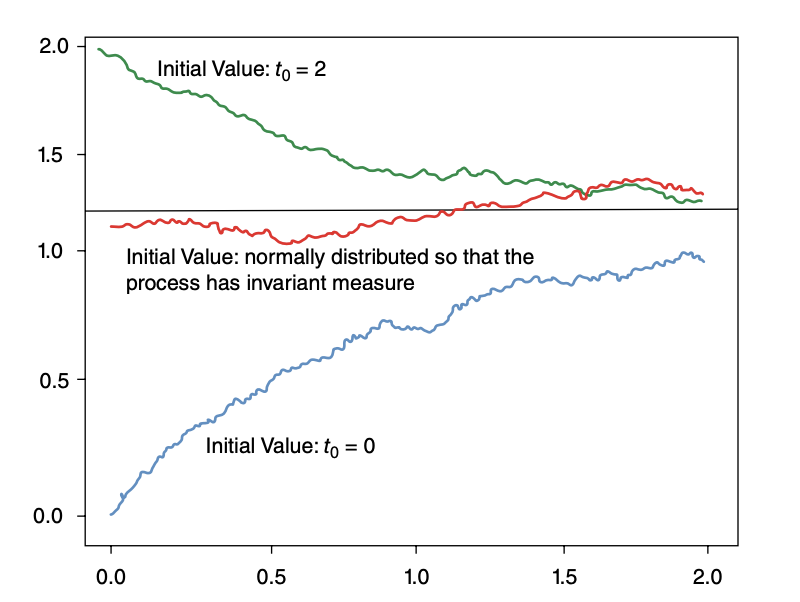
\includegraphics[width=1.0\textwidth]{im7}
    \caption{Ornstein-Uhlenbeck Process (Energy Tradink and Risk Management, Wiley 2014)}
    \label{fig:enter-label3}
\end{figure}



\subsection{Mean Reversion: Processo stocastico di Schwartz}

Prendiamo in considerazione l'equazione differenziale stocastica

\begin{equation}
    dS_t = \alpha (\mu_L - \ln(S_t)) S_t dt + \sigma_L S_t dW_{t} \label{eq:OI}
\end{equation}

dove:
\begin{itemize}
    \item $S_t$ = S(t) indica il prezzo spot all'istante t
    \item $S_0$ = S(0) indica il prezzo spot all'istante t = 0
    \item $\mu_L$ indica il valor medio di lungo periodo del prezzo ln($S_t$)
    \item $\sigma$ indica la volatilità (deviazione standard) di $S_t$
    \item $\alpha$ denota la velocità di \textit{mean reversion} e caratterizza la velocità con cui tali traiettorie si raggrupperanno intorno a $\mu_L$ nel tempo
    \item $W_t$ = W(t) processo di Wiener (o moto Browniano standard)
\end{itemize}



Il modello di Schwartz è un processo stocastico Ornstein-Uhlenbeck con l'aggiunta di una trasformata logaritmica sul prezzo spot. 

Anche questo processo è comunemente utilizzato nella modellazione dei prezzi spot dell'energia elettrica. Nella fatti specie, viene maggiormente adattato per gestire le anomalie nei prezzi, come picchi improvvisi, interruzioni, stagionalità e variazioni tra diverse regioni geografiche della rete nazionale (Clewlow e Strickland 2000).

Ad esempio, durante le ore di picco della domanda, il costo dell'elettricità può aumentare considerevolmente. Al contrario, durante le ore di minor consumo, come tarda notte ad esempio, il prezzo può diminuire. Inoltre, possono verificarsi ampie fluttuazioni dei prezzi tra le ore di picco e le ore di minor consumo, generando così importanti dislivelli, anche nel corso della medesima giornata. Per tener conto di questa volatilità, i modelli possono essere adattati per stimare un valore previsto normalizzato o diffuso nel tempo che tenga conto di possibili salti continui.

La SDE \eqref{eq:OI} presenta la seguente soluzione:

\begin{equation}
S_t = \exp \left\{\ln(S_0) e^{-\alpha t} + \left(\mu_L - \frac{\sigma^2}{2\alpha}\right) \left[1 -  e^{-\alpha t}\right] + \int_{0}^{t} e^{\alpha (x-t)} \sigma \, dW(x)\right\}
\end{equation}

dove:
\begin{itemize}
    \item $S_t$ = S(t) indica il prezzo spot all'istante t
    \item $S_0$ = S(0) indica il prezzo spot all'istante t = 0
    \item $\mu_L$ indica il valor medio di lungo periodo del prezzo ln($S_t$)
    \item $\sigma$ indica la volatilità (deviazione standard) di $S_t$
    \item $\alpha$ denota la velocità di \textit{mean reversion} e caratterizza la velocità con cui tali traiettorie si raggrupperanno intorno a $\mu_L$ nel tempo
    \item $W_t$ = W(t) processo di Wiener (o moto Browniano standard)
\end{itemize}



\section{Analisi dei prezzi a termine: forward e future}


Come intravisto precedentemente, il \textit{prezzo a termine} è un prezzo predeterminato di consegna per una merce, una valuta o un'attività finanziaria sottostante, deciso dall'acquirente e dal venditore, il quale viene pagato in una data predeterminata futura (Iris Mack, 2014). Solito dei contratti forward/futures stipulati tra un cliente e un produttore di energia elettrica, per acquistare (vendere) una determinata quantità di elettricità ad un prezzo concordato, con lo scopo di coprirsi a possibili rincari a breve termine. Nello specifico, i partecipanti ai mercati finanziari utilizzano contratti forward per condividere il rischio di rialzo del prezzo, pagando un ulteriore premio pur di abbassare la percentuale di rischio stesso a loro carico.
Nello specifico, quando due parti sottoscrivono un contratto forward o futures, non avviene alcuno scambio di denaro. Alla data di stipula, t, il valore del contratto è zero perché il prezzo pattuito per lo scambio del bene sottostante (K) è uguale al prezzo forward $(Ft,T)$, con T che rappresenta la data di consegna. Il prezzo forward, quindi, rappresenta sia il prezzo futuro prefissato al quale l'acquirente dovrà pagare il venditore per ricevere una unità del bene sottostante, sia il prezzo equo che le parti attribuiscono durante le negoziazioni per quel particolare contratto. Con il passare del tempo, tuttavia, mentre il prezzo di consegna K rimane costante, il prezzo forward cambia in base alle aspettative future riguardo al prezzo spot del bene sottostante. Così, quel contratto, che all'inizio aveva un valore nullo a t, potrebbe assumere un valore positivo o negativo a seconda del nuovo prezzo forward che le parti o il mercato ritengono equo per negoziare un contratto con condizioni simili.

Da qui è possibile definire una distinzione tra \textit{contratto forward finanziario} e \textit{contratto forward fisico}. Il primo prevede che la materia prima scambiata (per esempio l'elettricità) non venga consegnata fisicamente; il secondo, al contrario, prevede il conseguimento fisico della materia prima scelta, garantendo la possibilità di negoziare tali contratti sia in borsa, sia attraverso transazioni \textit{over the counter} (OTC).


Nel mondo finanziario, la relazione tra prezzo spot e prezzo forward per materie prime scambiate fisicamente può essere determinato con la seguente formula:

\begin{equation}
    F(t,T) = e^{r(T-t)} S(t)
\end{equation}

Dove:
\begin{itemize}
    \item F(t,T) è il prezzo forward del contratto a termine 
    \item r rappresenta il tasso di interesse privo di rischio
    \item S(t) rappresenta il prezzo spot dell'attività sottostante
\end{itemize}
    
Questa espressione è formulata sotto l'ipotesi di assenza di arbitraggio\footnote{In economia e finanza, un arbitraggio è un'operazione che consiste nell'acquistare un bene o un'attività finanziaria su un mercato rivendendolo su un altro mercato, sfruttando le differenze di prezzo al fine di ottenere un profitto (Wikipedia)}. Nel caso in cui $F(t,T)$ risultasse maggiore di $e^{r(T-t)} S(t)$ allora si potrebbe trarre profitto dall'acquisto al tempo $t$ dell'attività sottostante prendendo in prestito il denaro sufficiente ($S(t)$) al tasso privo di rischio $r$ e rivendendo tale bene al prezzo forward. Caso contrario, se $F(t,T)$ risultasse minore di $e^{r(T-t)} S(t)$ allora si potrebbe generare un guadagno certo, privo di rischio, semplicemente vendendo allo scoperto\footnote{Vendere allo scoperto significa vendere un titolo che non si possiede per ricomprarlo successivamente, poiché si scommette sul suo ribasso. Un’operazione generalmente considerata rischiosa, ma che può portare benefici significativi alla performance degli investimenti coprendo il portafoglio negli scenari ribassisti. Più nello specifico, questa strategia finanziaria consiste nel vendere oggi un asset (es. azioni) che non si possiede e che si è preso a prestito, nella convinzione che il valore diminuisca, per riacquistarli successivamente a un prezzo inferiore in modo da restituirle al broker e trarne profitto (orafinanza.it)} la materia prima al prezzo spot, investendo successivamente la somma di denaro ricavata nell'acquisto della stessa tipologia di bene al prezzo forward $F(t,T)$.


Il primo caso, il mercato dei futures assume il nome di \textbf{\textit{mercato in contango}} mentre il secondo assume il nome di \textbf{\textit{mercato in backwardation}}. A differenza dei classici mercati, nel mercato delle commodities parlare di \textit{contango} non risulta un'eventualità ma mera normalità. Questo è dovuto all'abbassamento del premio richiesto per l'acquisto della merce quando la scadenza dei futures si avvicina, generando così un avvicinamento del prezzo forward al prezzo spot, portando il mercato "in contango". In altre parole, il prezzo per consegnare una merce in una data futura risulta quasi sempre maggiore di quello richiesto per la medesima consegna immediata. Tale aumento è causato dai costi di gestione legati alle materie prime scambiate, naturalmente intese come beni fisici e tangibili (ciò non si verifica, per esempio, nel caso di asset finanziari, i quali non richiedo costi di gestione o trasporto).
L'esatto opposto si osserva nella \textit{backwardation}, molto meno comune nel mercato interessante le materie deperibili e tangibili, dove il prezzo spot della risorsa, a scadenza, è inferiore a quello atteso. Nello specifico, si tratta di una vera e propria alterazione del prezzo, dovuta principalmente a fattori esterni che generano incertezza e, quindi, un relativo abbassamento del valore finale. Può accadere per esempio che la domanda aumenti bruscamente in seguito ad un timore pressante rilegato ad una possibile carestia nell'immediato futuro, estreme siccità in corso, ecc. In altre parole, è possibile intravedere questo effetto quanto un fattore geopolitico spinge ad investire nel presente, andando incontro ad un relativo aumento dei costi, pur di non rischiare di rimanere a mani vuote in istanti futuri. 

\begin{center}
\includegraphics[width=0.8\textwidth]{im8}
\end{center}

Nel caso in cui le materie prime risultassero beni di consumo come le principali commodities energetiche (petrolio greggio e gas naturale), la formulazione precedente non risulta adeguata, in quanto andrebbero considerati ulteriori elementi. Nello specifico, bisogna tener conto sia del costo sostenuto per conservare nel tempo la merce in possesso, sia del tasso di convenienza, il quale esprime il beneficio a vantaggio del possessore nel detenere il bene di consumo per via diretta, al contrario dell'acquirente che assume una posizione lunga sul contratto forward sul medesimo bene.

Per una materia prima, quindi, come il petrolio, che può essere sia consumato che trattato come un normale titolo finanziario per scopi di investimento, è più appropriato esprimere la relazione tra il prezzo forward e il prezzo spot attraverso la seguente equazione:

\begin{equation}
    F(t,T) = e^{(r+s-y)(T-t)} S(t)
\end{equation}

Dove:

\begin{itemize}
    \item r rappresenta il tasso di interesse privo di rischio
    \item S(t) rappresenta il prezzo spot dell'attività sottostante
    \item F(t,T) rappresenta il prezzo a termine del sottostante al tempo t con scadenza al tempo finale T
    \item y rappresenta il rendimento di convenienza
    \item s rappresenta il costo di stoccaggio della materia prima
\end{itemize}

Tale formulazione risulta ottimale nella gestione della maggior parte dei beni scambiati nei mercati finanziari, fatta eccezione per il mercato dell'energia elettrica. Come è stato accennato precedentemente (si veda il capitolo 1), l'impossibilità di conservare questa materia prima, essendo essa immagazzinabile, e, quindi, non trasferibile nel tempo, comporta l'inapplicabilità delle formulazioni sopra descritte, in quanto non si potrebbe stimare un vero e proprio rendimento di convenienza (y) poiché risulta complesso accumulare scorte di elettricità. 



\chapter{Soluzioni per il prezzaggio dei derivati esotici energetici}

Nelle sezioni precedenti, abbiamo esaminato modelli utilizzati per la valutazione di due categorie di derivati energetici noti come \textit{plain vanilla}: futures e forwards. Tuttavia, il mondo dei derivati energetici è molto più complesso e variegato di quanto questi strumenti standard possano rappresentare. 

In questo capitolo, ci introdurremo nel mondo affascinante dei derivati energetici esotici, che rappresentano una classe di strumenti finanziari più sofisticata e adattabile alle esigenze specifiche degli operatori del mercato energetico.
I derivati esotici, a differenza dei derivati plain vanilla, incorporano caratteristiche uniche e complesse che consentono agli operatori di sfruttare una vasta gamma di scenari e condizioni di mercato. Questi strumenti sono stati progettati per affrontare specifiche sfide e opportunità che possono emergere nell'industria dell'energia, come la gestione di rischi particolarmente complessi o la scommessa su eventi insoliti.

Nel corso di questo paragrafo, esploreremo varie tipologie di derivati esotici, ne analizzeremo le caratteristiche distintive e impareremo come valutarli. Vedremo come tali strumenti possano essere utilizzati per mitigare rischi o sfruttare opportunità uniche all'interno del settore energetico. 


\section{Opzioni Asiatiche}


Le opzioni Asiatiche (Asian option), conosciute anche sotto il nome di opzioni sul prezzo medio (APO), rientrano nella categoria delle opzioni esotiche, ovvero una particolare tipologia di contratti derivati basati su condizioni più complesse rispetto alle metodologie classiche intraviste nelle opzioni \textit{plain vanilla}, come date di esercizio differenti o meccanismi di pagamento non lineari. Dal punto di vista energetico una delle opzioni più ampiamente negoziate nel settore, in particolare nei mercati petroliferi e del gasolio da riscaldamento,  risultando ottime alternative nella valutazione e copertura dei rischi associati ai flussi di cassi periodici.

Nello specifico, il principale utilizzo delle APO nel settore energetico è dovuto principalmente a due fattori fondamentali:
 \begin{itemize}

\item \textbf{Riflessione delle Transazioni Energetiche Realistiche}: Le opzioni asiatiche riescono a catturare la complessità delle transazioni energetiche reali. Queste transazioni, che coinvolgono solitamente consegne multiple nell'arco di un mese, non sono facilmente rappresentate da opzioni \textit{plain vanilla} europee basate su un singolo prezzo di scadenza. Le opzioni asiatiche, grazie alla loro caratteristica di media del profitto, rispecchiano in modo più accurato l'aspetto commerciale tipico di gran parte delle negoziazioni energetiche, in cui il prezzo è calcolato sulla base di una media temporale anziché un prezzo unico alla scadenza.

\item \textbf{Costo Inferiore rispetto alle Opzioni Vanilla}: Un ulteriore vantaggio delle opzioni asiatiche è il loro costo solitamente inferiore rispetto alle opzioni \textit{plain vanilla} europee con parametri simili, come data di scadenza, prezzo sottostante e volatilità. Questa convenienza è il risultato diretto della natura delle Asian option. La media dei prezzi sottostanti nel tempo tende a mitigare gli estremi picchi di prezzo e a smorzare la volatilità, rendendole strumenti di gestione del rischio relativamente più accessibili dal punto di vista economico.
 \end{itemize}

Le APO si dimostrano estremamente utili, per esempio, nell'ambito della copertura dei costi del bunker oil\footnote{Con il termine di bunker oil ci si riferisce a qualsiasi tipo di olio combustibile impiegato per la locomozione delle navi. Il termine "bunker" deriva dal nome inglese dei contenitori nei quali è immagazzinato, in particolare i \textit{bunker tank} delle imbarcazioni e i bunker nei siti portuali.} in situazioni in cui le operazioni quotidiane, come il viaggio di una nave, comportano un consumo continuo di carburante. Settori quali il trasporto marittimo, le compagnie di crociere e le aziende di noleggio sono spesso soggetti a fluttuazioni nei prezzi del carburante, che possono avere un impatto significativo sui loro bilanci e sui flussi di cassa. In questo contesto, l'utilizzo di opzioni asiatiche offre un meccanismo flessibile per gestire il rischio associato alle oscillazioni dei prezzi del carburante, consentendo alle aziende di stabilizzare i loro costi e pianificare in modo più efficace le loro operazioni finanziarie.

I primi contratti di opzioni asiatiche furono emessi nel 1987 a Tokyo, in Giappone, grazie alla formulazione di due dipendenti di Bankers Trust\footnote{Bankers Trust era una storica organizzazione bancaria americana. La banca si è fusa con Alex. Brown $\&$ Sons nel 1997 prima di essere acquisita da Deutsche Bank nel 1999.}, David Spaughton e Mark Standish, per le opzioni rilegate al prezzo medio del petrolio greggio. Per quanto riguarda il funzionamento di questi contratti derivati, il valore finale delle opzioni asiatiche dipende sempre dal valore dell'attività sottostante S, ma in questo caso non è considerato unicamente alla data di scadenza, ma anche in momenti precedenti alla scadenza stessa. In altri termini, si prende in considerazione, come payoff finale, la media (aritmetica o geometrica) dei prezzi del sottostante assunti durante il periodo contrattuale. Per questa ragione, è possibile ritrovare questi strumenti anche sotto il nome di opzioni \textit{path dipendent} (dipendenti dal percorso).


\begin{figure}[htbp]
    \centering
    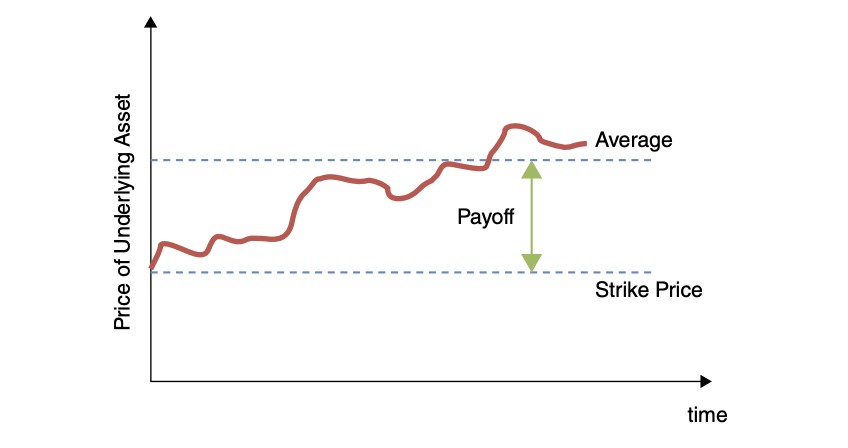
\includegraphics[width=0.8\textwidth]{im9}
    \caption{Opzione call Asiatica}
    \label{fig:grafico}
\end{figure}

Esistono due tipologie principali di Opzioni Asiatiche:

\begin{itemize}
    \item \textbf{a strike variabile}: le opzioni asiatiche con strike variabile pagano la differenza tra il prezzo medio registrato dall'attività sottostante energetica e il prezzo spot. Tali contratti consentono al detentore dell'opzione di acquistare o vendere gas o energia a pronti ad un prezzo di esercizio predeterminato all'inizio del mese.
    \item \textbf{a strike fisso}: Le opzioni asiatiche a strike fisso consentono al detentore dell'opzione di acquistare o vendere un'attività sottostante a un prezzo di esercizio stabilito in anticipo. Tale prezzo fisso è basato sulla media dei prezzi dell'attività sottostante durante un periodo specifico, e il pagamento avviene in base alla differenza tra questo valore e il prezzo spot dell'attività al momento dell'esercizio. 
\end{itemize}

La determinazione del valore medio è soggetta a diversi parametri che ne condizionano il risultato, tra cui la durata temporale considerata (che può corrispondere all'intera vita dell'opzione o a un suo segmento), la tipologia di media scelta (che può essere sia aritmetica che geometrica), l'assegnazione del peso ai vari prezzi in funzione dell'importanza del periodo di riferimento, e il metodo di campionamento utilizzato (che può essere continuo o discreto).

Un'ulteriore classificazione delle opzioni asiatiche è la seguente:

\begin{itemize}
    \item \textbf{Opzioni asiatiche discrete}: Le opzioni asiatiche discrete sono contratti finanziari derivati in cui il prezzo di esercizio è determinato dalla media dei prezzi dell'attività sottostante in un insieme discreto di momenti durante il periodo di osservazione. A differenza delle opzioni asiatiche continue, le opzioni asiatiche discrete prendono in considerazione solo un numero limitato di prezzi di riferimento. In altre parole, durante il periodo di osservazione, che può essere suddiviso in segmenti temporali specifici (ad esempio, giorni, settimane o mesi), vengono registrati i prezzi dell'attività sottostante in ciascun intervallo temporale. Il prezzo di esercizio è quindi determinato dalla media dei prezzi durante il periodo specifico.
    
    \item \textbf{Opzioni asiatiche continue}: Le opzioni asiatiche continue, presentano anch'esse un prezzo di esercizio determinato dalla media continua dei prezzi dell'attività sottostante durante un periodo di osservazione specifico. A differenza delle opzioni asiatiche discrete, però, le opzioni asiatiche continue calcolano la media in modo continuo, lungo l'intero periodo di osservazione. Nello specifico, i prezzi dell'attività sottostante vengono monitorati costantemente, e il prezzo di esercizio viene determinato dalla media aritmetica/geometrica continua di questi prezzi durante il periodo specificato. Questo rende le opzioni asiatiche continue meno sensibili alle fluttuazioni dei prezzi a breve termine rispetto alle opzioni a strike fisso tradizionali.
    
    \item \textbf{Opzioni asiatiche forward-start}: Le opzioni asiatiche forward-start combinano le caratteristiche delle opzioni asiatiche e delle opzioni forward-start\footnote{In finanza, un'opzione forward-start (di avvio anticipato) è un'opzione che inizia a una data futura specificata con una data di scadenza fissata più avanti nel futuro (Wikipedia)}. Tali strumenti derivati sono progettati per fornire agli investitori una maggiore flessibilità nella gestione del rischio e delle opportunità di speculazione, in quanto presentano caratteristiche come:

    \begin{enumerate}
        \item Strike price iniziale differito: il prezzo di esercizio non viene definito nell'istante di chiusura del contratto, ma inizia a essere determinato solo in un secondo momento, in genere a una data futura specificata. Questo differimento nel prezzo di esercizio consente agli investitori di adattarsi meglio alle condizioni di mercato cambianti.
        \item Scadenza flessibile: la scadenza delle opzioni asiatiche forward-start può essere impostata in modo flessibile per soddisfare le esigenze dell'investitore. Questo offre l'opportunità di personalizzare ulteriormente il contratto in base alle aspettative e alle strategie finanziare.
    \end{enumerate}

\end{itemize}

Le Asian option presentano un alto livello di complessità nel prezzaggio sia analitico che numerico. Pur essendo state al centro di molte attenzioni negli anni recenti, in termini di ricerca, non esiste ancora oggi una vera e propria tecnica che risulti ottimale per prezzare le opzioni Asiatiche per tutte le scelte dei parametri di mercato. Per questo motivo è opportuno ricorrere alle formulazioni presenti nel modello di Black \& Scholes classico, a singolo fattore di rischio, basato su un moto Browniano standardizzato.
La formulazione di B\&S è la seguente:

\begin{equation}
    dS_t = rS_t dt + \sigma S_t dW_t, \quad t \geq 0
\end{equation}

dove $W_t$ ($t>0$) è un Moto Browniano standard, $\sigma$ rappresenta la volatilità (costante) r è il tasso d'interesse senza rischio (costante) e infine $S_0$ è il prezzo iniziale. L'equazione (9) può essere riscritta nella equazione:

\begin{equation}
    S_t = S_0 e^{\mu t + \sigma W_t}, \quad t \geq 0
\end{equation}

dove $\mu = r - \frac{\sigma^2}{2}$. Per ogni $T > 0$

\begin{equation}
    A_c = \frac{1}{T} \int_{0}^{T} S_t \, dt
\end{equation}

è il prezzo medio dell'attività sottostante, calcolato utilizzando una media aritmetica, nel lungo periodo [0,T].
Nel caso discreto, fissando un n come numero di osservazioni registrate, considerando sempre T come data di scadenza finale dell'opzione, il valore medio assunto dall'attività sottostante, sempre utilizzando una media aritmetica per il calcolo, è pari a:

\begin{equation}
    A_d = \frac{1}{n} \sum_{k=1}^{n} S_{t_{k}}
\end{equation}


Sulla base di queste formulazioni, è ora possibile definire il valore di un opzione Asiatica di tipo call con prezzo di esercizio maggiore di zero e scadenza fissata in T:

\begin{equation}
(C_A) \, ^c = e^{-rT}\mathbb{E}\left[\max(A_T - K, 0)\right]
\end{equation}

Un altra tipologia di opzione con la media sul prezzo è l'opzione Asiatica di tipo geometrico. Ovvero, prendendo in considerazione il caso discreto, il payoff dipende dalla media geometrica del prezzo dell'attività sottostante. Anche in questo caso è possibile distinguere due formulazioni, in funzione ci ritrovassimo nel discreto o nel continuo. In particolar modo, per quanto concerne il caso discreto, si ha la seguente formulazione:

\begin{equation}
    G_d = \left(\prod_{i=1}^{N} S_i\right)^{\frac{1}{N}} \label{eq:geom}
\end{equation}

Mentre, nel caso continuo, considerando sempre l'intervallo [0,T], si ottiene:

\begin{equation}
    G_c = \exp\left(\frac{1}{T} \int_{0}^{T} \log(S(u)) \, du\right)
\end{equation}


Sotto le medesime condizioni definite in precedenza riguardo il prezzo di esercizio e la scadenza fissata, il valore call e il valore put dell'opzione a media geometrica è data da:



\begin{equation}
    (C_G)^d = e^{-rT}\mathbb{E}\left[\max(G_N - K, 0)\right]
    \end{equation}
    \begin{equation}
    (P_G)^d = e^{-rT}\mathbb{E}\left[\max(K - G_N, 0)\right]
\end{equation}


Nei mercati finanziari, gran parte delle opzioni asiatiche negoziate utilizza la media aritmetica come parametro di riferimento. Tuttavia, la considerazione della media geometrica nella valutazione delle opzioni asiatiche è altrettanto significativa. Questo è dovuto al fatto che, a differenza della media aritmetica, la media geometrica consente l'uso di formule chiuse per la valutazione. Questa considerazione ha portato allo sviluppo di uno dei modelli maggiormente utilizzati nella pratica per valutare le opzioni asiatiche, noto come il \textbf{modello di Vorst}.

Il modello di Vorst si basa sull'idea di utilizzare la media geometrica come approssimazione della media aritmetica delle osservazioni dei prezzi dell'asset sottostante. Tuttavia, Vorst tiene conto dell'effetto dell'approssimazione attraverso una correzione dello strike price, come sarà descritta in seguito. Quindi, nella sostanza, si assume che il valore finale di un'opzione call asiatica possa essere espresso nella seguente forma: 

\begin{equation}
    \max\left(\frac{1}{n} \sum_{i=1}^{n} (S_{t_i} - K); 0\right)
\end{equation}
\begin{equation}
    \max\left((\prod_{i=1}^{n} S_{t_i})^\frac{1}{n} - K; 0\right)
\end{equation}

dove:

\begin{align*}
\frac{1}{n} \sum_{i=1}^{n} S_{t_i} &= \text{media aritmetica dei prezzi} \\
\left(\prod_{i=1}^{n} S_{t_i}\right)^{\frac{1}{n}} &= \text{media geometrica dei prezzi}
\end{align*}

Da qui si può dedurre che il valore corrente di un opzione asiatica di tipo call può essere scritta come: 

\begin{equation}
    C_{AS} = e^{-r(t_n - t_0)} E\left[\max\left(\left(\prod_{i=1}^{n} 
    S_{t_i}\right)^{\frac{1}{n}} - K; 0\right)\right]
\end{equation}

È utile notare come la preferenza nell'uso della media geometrica, rispetto alla media aritmetica, sia obbligatoria qualora si voglia ricorrere ad una forma di valutazione chiusa, ricavata per esempio dal modello di Black \& Scholes, in quanto la somma di variabili stocasticamente indipendenti, che seguono un andamento lognormale se prese singolarmente, non si distribuisce nella medesima legge, cosa che invece non si verifica se si adotta l'utilizzo della geometrica per la valutazione media dei prezzi.

In funzione di questa problematica, Vorst ha proposto la seguente formulazione, intesa come possibile variante del modello di B\&S, per la valutazione (sempre in forma chiusa) di una Asian option di tipo call:

\begin{equation}
    C_{AS} = e^{-r(t_n - t_0)} \left( e^{\mu_{lg} + \frac{\sigma_{lg}}{2}} N(d) - KN\left(d - \sqrt{\sigma_{lg}}\right) \right)
\end{equation}

dove:

\begin{align*}
    d = \frac{\mu_{lg} - \ln(K) + \sigma_{lg}}{\sqrt{\sigma_{lg}}}
\end{align*}

mentre i termini $\mu_{lg}$ e $\sigma_{lg}$ rappresentano rispettivamente la media e la varianza del logaritmo della media geometrica, rispettivamente uguali a:

\begin{equation}
    \mu_{lg} = \ln(S_{t_0}) + \frac{1}{n} \sum_{i=1}^{n}(r - q - \frac{\sigma^2}{2}) (t_i - t_0)
\end{equation}

\begin{equation}
    \sigma_{lg} = \frac{\sigma^2}{n^2} \sum_{i=1}^{n} \sum_{j=1}^{n}\min\left(t_i - t_0; t_j - t_o\right)
\end{equation}


dove:

\begin{itemize}
    \item $S_{t_0}$: Prezzo all'istante di valutazione.
    \item $q$: Dividend yield.
    \item $\sigma$: Volatilità del titolo sottostante.
    \item $t_0$: Data di valutazione.
    \item $t_i$: Istante i-esimo di rilevazione.
    \item $r$: Tasso risk-free.
\end{itemize}

Una seconda correzione suggerita da Vorst riguarda il livello del prezzo di esercizio K per la differenza tra il valore della media aritmetica e quello della media geometrica in riferimento sempre alle rilevazioni dei prezzi dell'attività sottostante, la quale risulta, nel caso geometrico, sempre minore o al limite equivalente al medesimo calcolo utilizzando la media aritmetica. Quindi, lo strike price corretto suggerito da Vorst assume la seguente forma:

\begin{equation}
    K^* = K - \left[ \mathbb{E}\left(\frac{1}{n}\sum_{i=1}^{n}S_{t_i}\right) - \mathbb{E}\left(\left(\prod_{i=1}^{n}S_{t_i}\right)^\frac{1}{n}\right) \right]
\end{equation}

dove i rispettivi valori attesi nel caso aritmetico e nel caso geometrico sono i seguenti:

\begin{align*}
   \mathbb{E}\left(\frac{1}{n}\sum_{i=1}^{n}S_{t_i}\right) = S_{t_0} \cdot \frac{\sum_{i=1}^{n}e^{(r-q)\cdot(t_i - t_0)}}{n}
\end{align*}

\begin{align*} \mathbb{E}\left(\left(\prod_{i=1}^{n}S_{t_i}\right)^\frac{1}{n}\right) = e^{\mu_{lg} + \frac{\sigma_{lg}}{2}}
\end{align*}

Riconsiderando quindi il valore corretto del prezzo di esercizio, sostituendolo nella formulazione (4.13), si ottiene:

\begin{equation}
    C_{AS} = e^{-r(t_n - t_0)} \left( e^{\mu_{lg} + \frac{\sigma_{lg}}{2}} N(d) - K^*N\left(d - \sqrt{\sigma_{lg}}\right) \right)
\end{equation}

dove: 

\begin{align*}
     d = \frac{\mu_{lg} - \ln(K^*) + \sigma_{lg}}{\sqrt{\sigma_{lg}}}
\end{align*}
 Nel caso infine di un’opzione put asiatica, formula di valutazione `e la seguente:

\begin{equation}
    P_{AS} = e^{-r(t_n - t_0)} \left( e^{\mu_{lg} + \frac{\sigma_{lg}}{2}} N(d) - K^*N\left(d - \sqrt{\sigma_{lg}}\right) \right)
\end{equation}


\section{Opzioni Barriera}

Nel complesso panorama della gestione dei rischi nel settore energetico, le opzioni barriera rappresentano uno strumento finanziario innovativo ed efficace per mitigare l'esposizione ai rischi di prezzo e di mercato. Queste opzioni, conosciute anche come opzioni 'a barriera', sono state sviluppate per adattarsi alle specifiche esigenze delle aziende e delle organizzazioni coinvolte nell'industria dell'energia. 

Nello specifico, quando parliamo di Barrier Option (BO), ci riferiamo ad uno degli strumenti più antichi, appartenenti sempre alla categoria delle opzioni esotiche, ad esser stati negoziati sul mercato mondiale. Una prima opzione Call a barriera è stata negoziata sul mercato OTC americano nel 1967, ma lo sviluppo di questo strumento avverrà successivamente con l'emissione di ulteriori sotto-categorie alla fine degli anni ottanta, dando il via al completo sviluppo di ulteriori tecniche di copertura, soprattutto nel ramo energetico.

Le opzioni barriera presentano una caratteristica unica, in quanto possono attivarsi (knock-in) o disattivarsi (knock-out) quando il prezzo dell'attività sottostante raggiunge un valore specifico noto come "barriera" (indicata con H).

In ambito petrolifero, le aziende produttrici potrebbero utilizzare questi strumenti per coprirsi da possibili andamenti dei prezzi a ribasso, generando una possibile copertura qualora si palesasse una perdita di valore. Per esempio, se il prezzo attuale del petrolio è di \$50 a barile, e si acquista un'opzione barrier put con una barriera fissa \$40, l'opzione diventerà attiva solo se il prezzo del petrolio scende a \$40 o meno. In questo caso, l'opzione put diventerà profittevole, in quanto l'azienda potrà esercitarla per coprire le perdite dovute all'abbassamento del prezzo, nell'intervallo di tempo specifico del contratto.

Indipendentemente che siano opzioni di tipo call o put, le opzioni barriera possono essere suddivise in quattro categorie distintive:

\begin{itemize}
    \item \textit{Down-and-out}: Queste opzioni concedono al detentore il diritto, ma non l'obbligo, di comprare o vendere un asset sottostante a un prezzo prestabilito in partenza, a condizione che il prezzo $S_t$ di quell'asset non scenda al di sotto di un livello barriera concordato H, durante l'intera durata dell'opzione. In modo più specifico, una volta che il prezzo dell'asset sottostante scende al di sotto della barriera, l'opzione viene disattivata (knocked-out)
    \item \textit{Down-and-in}: Queste opzioni sono l'opposto delle opzioni barriera "down-and-out". Hanno valore solo se il prezzo dell'asset sottostante $S_t$ scende al di sotto della barriera H durante la durata dell'opzione. Se la barriera viene superata, il detentore dell'opzione "down-and-in" ha il diritto di acquistare o vendere l'asset al prezzo di esercizio K prestabilito alla data di scadenza.
    \item \textit{Up-and-out}: Queste opzioni presentano somiglianze con le opzioni barriera "down-and-out". Le opzioni "up-and-out" vengono disabilitate se il valore dell'asset sottostante supera la barriera predefinita, determinando così la perdita del diritto di esercizio da parte del possessore.
    \item \textit{Up-and-in}: Queste opzioni sono comparabili alle opzioni "down-and-in". La barriera H è posizionata al di sopra del prezzo attuale dell'asset sottostante $S_t$ e l'opzione sarà valida solo se il prezzo dell'asset raggiunge la barriera prima della scadenza.
\end{itemize}

Di norma, la barriera si trova quasi sempre nella regione \textbf{out-of-the-money} (OTM), ovvero posizionata al di sotto del prezzo di esercizio K previsto, valido per le opzioni call.  Da qui il nome di \textbf{standard barrier} (o regular barrier). Nel caso in cui le opzioni prevedano una barriera situata nella regione \textbf{in-the-money} (ITM), cioè presentino una barriera al di sopra del prezzo di esercizio K, assumono il nome di \textbf{reverse barrier}. 

A causa della presenza della barriera, che impone restrizioni sull'esercizio dell'opzione, i premi associati tendono ad essere più modesti rispetto a quelli delle opzioni europee standardizzate. Inoltre, la complessità delle BO può aumentare ulteriormente quando vi è una barriera discontinua (ad esempio, legata al tempo) e/o la possibilità di un \textit{rebate}\footnote{Consiste in un pagamento fisso, erogato dal detentore dell'opzione, quando l'asset sottostante $S_t$ raggiunge il livello della barriera H (per le knock-out), o nel caso non lo raggiunga mai (per le knock-in). Tale condizione può essere applicata, di per sé, a qualsiasi opzione barriera, ma solitamente la si ritrova nei contratti di opzione \textit{reverse barrier}.}. 

Il primo modello di \textit{pricing} delle opzioni barriera fu ideato da Merton nel 1973. Si trattava di una valutazione effettuata sulle \textit{down-and-out}, basata sulla risoluzione di un'equazione differenziale stocastica condizionata. Nel 1991, contemporaneamente alla pubblicazione dei brevi articoli di Hudson e Benson, Rubinstein e Reiner (1991) resero disponibile una completa valutazione utilizzando un approccio simile a quello di Black \& Scholes per tutte le varie tipologie di opzioni barriera standard esistenti. Successivamente, nel 1994, Boyle e Lau (1994) adottarono un metodo binomiale, meno sofisticato ma comunque efficace, per raggiungere gli stessi obiettivi. Nel corso degli anni successivi, la letteratura sull'argomento ha registrato un notevole sviluppo, ma senza introdurre innovazioni di rilievo rispetto agli studi citati in precedenza. 

Prendendo in considerazione la metodologia proposta da Hudson, Benson, Rubinstein e Reiner, il valore di una call di tipo \textit{down-and-out} può essere suddivisa nella somma di tre elementi che rappresentano:

\begin{enumerate}
    \item il valore di un'opzione call ordinaria con caratteristiche equivalenti
    \item la riduzione del prezzo dovuta alla presenza della barriera nel contratto
    \item il valore del rimborso eventuale erogato (qualora sia previsto il \textit{rebate})
\end{enumerate}

Nel caso in cui la barriera H risulti fissa e che la quota di rimborso prevista R non cambi nel tempo, considerando un prezzo di esercizio K e il valore dell'asset sottostante di partenza $S_0$ minori della barriera, si può dimostrare che il valore di una call all'istante t=0 è il seguente:

\begin{equation}
   C_{\text{DAO}} = \left[S_0 N(a_1) - K e^{-rT} N(a_2)\right]\label{eq:barrier}
\end{equation}
\begin{align*}
       - \left[S_0 \left(\frac{H}{S_0}\right)^{2(\eta + 1)} N(b_1) - K e^{-rt} 
   \left(\frac{H}{S_0}\right)^{2\eta} N(b_2)\right] 
\end{align*}
\begin{align*}
       + \left[R \left(\frac{H}{S_0}\right)^{\eta + \gamma} N(c_1) + R \left(\frac{H}{S_0}\right)^{\eta - \gamma} N(c_2)\right]
\end{align*}

\begin{equation}
       P_{\text{DAOP}} = \left[K e^{-rT} N(-a_2) - S_0 N(-a_1)\right] \label{eq:barrier1}
\end{equation}
\begin{align*}
      - \left[K e^{-rT} \left(\frac{H}{S_0}\right)^{2\eta} N(-b_2) - S_0 \left(\frac{H}{S_0}\right)^{2(\eta + 1)} N(-b_1)\right]
\end{align*}
\begin{align*}
       + \left[R \left(\frac{H}{S_0}\right)^{\eta - \gamma} N(-c_2) + R \left(\frac{H}{S_0}\right)^{\eta + \gamma} N(-c_1)\right]
\end{align*}

dove: 

\begin{multicols}{2} % Dividi in due colonne
\begin{align*}
\begin{aligned}
&\eta = \frac{r}{\sigma^2} - \frac{1}{2} 
\end{aligned}
\end{align*}
\columnbreak % 
\begin{align*}
\begin{aligned}
\\
&\gamma = \sqrt{\eta^2 + 2\frac{r}{\sigma^2}} \\
\end{aligned}
\end{align*}
\end{multicols}

\begin{multicols}{2} % Dividi in due colonne
\begin{align*}
\begin{aligned}
&a_1 = \frac{\log(S_0/X)}{\sigma\sqrt{T}} + (1 + \eta)\sigma\sqrt{T}
\end{aligned}
\end{align*}
\columnbreak % 
\begin{align*}
\begin{aligned}
\\
&a_2 = a_1 - \sigma\sqrt{T} \\
\end{aligned}
\end{align*}
\end{multicols}

\begin{multicols}{2} % Dividi in due colonne
\begin{align*}
\begin{aligned}
&b_1 = \frac{\log\left(H^2/S_0K\right)}{\sigma\sqrt{T}} + (1 + \eta)\sigma\sqrt{T}
\end{aligned}
\end{align*}
\columnbreak % 
\begin{align*}
\begin{aligned}
\\
&b_2 = b_1 - \sigma\sqrt{T} \\
\end{aligned}
\end{align*}
\end{multicols}

\begin{multicols}{2} % Dividi in due colonne
\begin{align*}
\begin{aligned}
&c_1 = \frac{\log\left(H/S_0\right)}{\sigma\sqrt{T}} + \gamma\sigma\sqrt{T}
\end{aligned}
\end{align*}
\columnbreak % 
\begin{align*}
\begin{aligned}
\\
&c_2 = c_1 - 2\gamma\sigma\sqrt{T} \\
\end{aligned}
\end{align*}
\end{multicols}


Per le restanti tre tipologie di opzione la formulazione risulta equivalente.

\section{Opzioni Lookback}

Le opzioni Lookback, anche conosciute come \textit{hindsight option} (opzione senno di poi), sono molto ambite nel settore elettrico, soprattutto durante i periodi in cui il valore dell'elettricità è fortemente influenzato dalle condizioni climatiche. Si tratta di un'ulteriore tipologia di derivato esotico che consente al possessore (holder) di esercitare il diritto di acquisto (Lookback call) o di vendita (Lookback put) della materia prima energetica sottostante al momento della scadenza. La peculiarità di queste opzioni risiede nella definizione dello \textit{strike price} K, il quale si basa sulle migliori condizioni di prezzo registrate durante il periodo contrattuale. In altre parole, al momento dell'esercizio, il titolare può sfruttare a suo vantaggio l'intera storia dell'attività sottostante (da cui il nome "lookback", tradotto come "guardare indietro"), selezionando il prezzo più favorevole possibile per la sua posizione.

Il profitto ottenuto dal detentore dipende sempre dalla differenza tra il prezzo di esercizio K fluttuante e il valore dell'attività sottostante a scadenza, ma, a differenza delle opzioni classiche \textit{plain vanilla}, ciò che rende questi strumenti particolarmente attraenti è l'elevata probabilità di esercizio, ricollegata alla possibilità di scelta delle condizioni più allettanti con le quali chiudere il contratto.

È possibile distinguere due tipologie differenti di opzioni Lookback:

\begin{itemize}
    \item \textbf{\textit{Fixed Lookback option}}: presenta un prezzo di esercizio K fisso, per cui la logica di acquistare o vendere in funzione del prezzo più conveniente si riferisce unicamente al titolo sottostante. È possibile trovare questo strumento anche sotto il nome di \textit{extrema lookback option}.
    In caso di opzione call, il detentore ha il diritto di rivedere lo storico dei prezzi e scegliere di esercitare nell'istante di maggiore potenziale di rendimento. Mentre, in caso di opzione put, naturalmente la scelta ricade sul valore minore presentato nel periodo di validità. 
    \item \textbf{\textit{Floating Lookback option}}: basato su un prezzo di esercizio K variabile, fissato alla scadenza, da cui deriva la logica di esercitare o meno in funzione del prezzo migliore. Nello specifico, l'investitore fissa lo \textit{strike price} K sulla base del prezzo più basso (per opzioni call) o di quello più alto (per opzioni put) assunte dall'asset finanziario sottostante durante il periodo di validità del contratto.
\end{itemize}

Di seguito sono riportate le formulazioni riguardanti i \textit{payoff}, sia nel caso call che nel caso put, per le due tipologie di contratto.
Nello specifico, per le \textit{Fixed Lookback option}:

\begin{equation}
    C_{\text{fx}} = \max (0; \max_{t < i < T} S_i - K)
\end{equation}
\begin{equation}
    P_{\text{fx}} = \max (O; K - \min_{t < i < T} S_i)
\end{equation}


mentre per le \textit{Floating Lookback option}:

\begin{equation}
    C_{\text{fl}} = \max (0; S_T - \min_{t < i < T} S_i) 
\end{equation}
\begin{equation}
    P_{\text{fl}} = \max (0; \max_{t < i < T} S_i - S_T)
\end{equation}

dove $\min_{t < i < T}$ e \(\max_{t < i < T}\) rappresentano rispettivamente il minimo e massimo valore raggiunto dall'attività sottostante $S_i$ durante la vita del contratto (ovvero nell'intervallo [0, T])

Se le \textit{fixed lookback option} risolvono il classico problema di uscita dal mercato per l'holder, ovvero il momento migliore per esercitare, le \textit{floating lookback option} aiutano a scegliere il momento ideale per entrare nel mercato e generare possibili profitti, in caso di mera attività speculativa, o per coprirsi da eventuali rischi connessi a cali di prezzo. 

Come si può evincere dalla loro definizione, questi strumenti sono una delle possibili soluzioni alle problematiche di \textit{hedging} aziendale connesse all'utilizzo dei titoli derivati, in particolar modo nel settore energetico, dove è maggiormente richiesta un'attenzione in più, soprattutto a causa delle nuove vicende geopolitiche, portatrici di instabilità e incertezza sui prezzi connessi al mercato dell'energia.
D'altro canto, a causa della loro struttura vantaggiosa, richiedono un costo di esecuzione molto elevato, e questo sarà notevolmente visibile nel prossimo capitolo, dove verranno proposti alcun. Questo inconveniente, però, può essere risolto stipulando un contratto \textit{partial lookback option}, il quale riduce sensibilmente la finestra temporale in cui è possibile scegliere il prezzo migliore, ma al contempo diminuisce il costo del premio connesso alla stipula del contratto.

Per la valutazione in forma chiusa, attraverso l'utilizzo del solito modello di Black \& Scholes, è possibile distinguere quattro formulazioni differenti, di seguito riportate.

\begin{enumerate}

    \item \textit{Floating lookback option}:
    \begin{equation}
    \begin{aligned}
        &C_{\text{Fl}} = S_t e^{-q \uptau} N(d_1) - S_{\text{min}} e^{-r\uptau} N(d_1) +\\
        &+\left[\frac{S_t e^{-r\uptau} \left(\frac{S_{\text{min}}}{S_t}\right)^{2\eta} N(-d_1 + 2\eta\sigma\sqrt{\uptau}) - e^{-q\uptau} S_t N(-d_1)}{2\eta}\right]
    \end{aligned}
    \end{equation}

\begin{equation}
    \begin{aligned}
        &P_{\text{Fl}} = S_{\max}e^{r\uptau}N(-d_2 + \sigma\sqrt{\uptau}) - S_t e^{-q\uptau} N(-d_2) -\\
        &- \left[\frac{S_t e^{-r\uptau} \left(\frac{S_{\text{max}}}{S_t}\right)^{2\eta} N(d_2 + 2\eta\sigma\sqrt{\uptau}) - e^{-q\uptau} S_t N(d_2)}{2\eta}\right]
    \end{aligned}
\end{equation}
\\
    \item \textit{Fixed lookback option}

\begin{equation}
    \begin{aligned}
        &C_{\text{Fx}} = S_t e^{-q\uptau}N(d_3) - K e^{-r\uptau} N(d_3 - \sigma\sqrt{\uptau}) +\\
        &+ \left[\frac{S_t e^{-q\uptau}N(d_3) - S_t e^{-r\uptau} \left(\frac{K}{S_t}\right)^{2\eta}N(d_3 - 2\eta\sigma\sqrt{\uptau})}{2\eta}\right]
    \end{aligned}
\end{equation}
\\
\begin{equation}
    \begin{aligned}
        &P_{\text{Fx}} = K e^{-r\uptau} N(-d_3 - \sigma\sqrt{\uptau}) - S_t e^{-q\uptau}N(-d_3) +\\
        &+ \left[\frac{S_t e^{-r\uptau}\left(\frac{K}{S_t}\right)^{2\eta}N(-d_3 + 2\eta\sigma\sqrt{\uptau}) - e^{-q\uptau}S_tN(-d_3)}{2\eta}\right]
    \end{aligned}
\end{equation}
    
\end{enumerate}

dove:

\begin{itemize}
    \item $S_{\text{min}}$: prezzo minimo registrato nel periodo di validità
    \item $S_{\text{max}}$: prezzo massimo registrato nel periodo di validità
    \item $S_t$: prezzo corrente del titolo sottostante
    \item $\uptau$: periodo residuo tra la data di scadenza e la data corrente di valutazione
    \item $\sigma$: volatilità del titolo sottostane
    \item $q$: dividend yeld
    \item $r$: tasso privo di rischio
    \item $\eta = \frac{(r - q)}{\sigma}$
    \item $d_1 = \frac{\ln\left(\frac{S_t e^{-q\uptau}}{S_{\text{min}}e^{-r\uptau}}\right) + \left(\frac{\sigma^2}{2}\right)\uptau}{\sigma\sqrt{\uptau}}$    
    \item $d_2 = \frac{\ln\left(\frac{S_t e^{-q\uptau}}{S_{\text{max}}e^{-r\uptau}}\right) + \left(\frac{\sigma^2}{2}\right)\uptau}{\sigma\sqrt{\uptau}}$
    \item $d_3 = \frac{\ln\left(\frac{S_t e^{-q\uptau}}{K e^{-r\uptau}}\right) + \left(\frac{\sigma^2}{2}\right)\uptau}{\sigma\sqrt{\uptau}}$
\end{itemize}




\chapter{Il metodo Monte Carlo}

Una metodologia alternativa per la valutazione di derivati energetici e, nello specifico, dei contratti di opzione introdotti nel capitolo precedente, è il metodo (o simulazione) Monte Carlo. La simulazione è una procedura che consente sia di seguire l'evolversi di un processo, sia di prevedere possibili scenari futuri, attraverso la costruzione di un modello che imita da vicino il sistema analizzato, o più semplicemente, generando dal modello numerosi campioni di casi possibili, sui quali studiare l'influenza del tempo sui risultati generati.

Introdotto circa alla metà degli anni 40 nell'ambito del Progetto Manhattan da Enrico Fermi, John von Neumann e Stanisław Marcin Ulam, presso il centro di ricerche nucleari di Los Alamos, assume il particolare nome di Monte Carlo in merito all'aleatorietà dei guadagni connessi al celebre casinò monegasco. Il metodo Monte Carlo è ampiamente utilizzato in diversi settori, come la fisica, l'ingegneria, l'economia e la statistica. Si basa sull'utilizzo di numeri casuali per simulare eventi probabilistici e ottenere stime o approssimazioni di quantità di interesse. 

È per definizione un metodo \textbf{stocastico} per il calcolo numerico di quantità deterministiche. Nello specifico, supponiamo di voler stimare una quantità generica $\beta$, equivalente al valore atteso di una v.a. X:

\begin{equation}
    \beta = \mathbb{E}(X)
\end{equation}

Supponiamo in aggiunta di lavorare al di sopra di un opportuno spazio di probabilità $(\Omega, \mathit{F}, \mathbb{P})$, dove $X : (\Omega, \mathit{F}) \rightarrow (\mathbb{R}^{d}, \mathit{B}(\mathbb{R}^{d}))$, e il simbolo $\mathbb{E}$ denota il valore atteso sotto $\mathbb{P}$. Immaginiamo adesso che X abbia legge di probabilità $\Gamma$, con X naturalmente integrabile, e sia $\{X^{n}\}_{n}$ una successione di v.a. indipendenti, tutte con medesima legge distributiva. Sulla base della \textbf{Legge dei Grandi Numeri}\footnote{La legge dei Grandi numeri afferma che, se prese in considerazione una successione di campioni casuali i.i.d. (indipendenti ed identicamente distribuiti) $X_1, X_2, ..., X_n$ con valore atteso $\mathbb{E}(X_i) = \mu_x$ e varianza $VAR(X_i) = \sigma^2 < \infty$, per ogni costante $c > 0$, si ha:

\begin{equation*}
\mathbb{P}(|\overline{X} - \mu_x| < c) \rightarrow 1 \quad \text{per } n \rightarrow \infty
\end{equation*}
ovvero, la probabilità che la media campionaria $\overline{X}$ coincida con la media della popolazione $\mu_x$, si avvicina sempre di più al valore unitario (certo) all'aumentare del numero dei campioni n.}, si ottiene: 

\begin{equation}
    \hat{\beta} := \frac{1}{N}\sum_{n=1}^{N}{X^{n}} \overset{N \to \infty}{\xrightarrow{}} \mathbb{E}(X) = \beta
\end{equation}

Quindi, una buona approssimazione del valore di $\beta$ si ricava calcolando la media empirica di un discreto numero di v.a. indipendenti con legge distributiva equivalente alla legge di probabilità di X. Questo è il metodo Montecarlo.

Messo in pratica, questo algoritmo si implementa attraverso poche righe di codice, utilizzando un qualsiasi ambiente di programmazione e calcolo numerico (come R o MATLAB), ma solo e unicamente nel caso in cui sia possibile simulare v.a. con legge distributiva $\Gamma$. Inoltre, la stima di $\hat{\beta}$ è solitamente soggetta ad una problematica principale. Nello specifico, essendo $\hat{\beta}$ per definizione una variabile aleatoria, è sostanzialmente improbabile che, una volta generato e inviato il codice, venga riprodotto uno stesso risultato. In altre parole, facendo girare l'algoritmo più volte, fissando un valore elevato di N, si possono ottenere stime differenti per $\beta$.

I metodi Monte Carlo trovano in ambito finanziario una naturale applicazione e vengono principalmente utilizzati per la risoluzione numerica dei problemi di prezzaggio e copertura dei titoli derivati. Con riferimento alla valutazione di opzioni finanziarie, la simulazione Monte Carlo è particolarmente adatta alle opzioni di tipo europeo (esercitabili, cioè, solo a scadenza) e alle opzioni sentiero dipendenti, ovvero le opzioni \textit{path dipendent}, oggetto di interesse del capitolo precedente. Nello specifico, l'uso della simulazione per stimare il prezzo di un'opzione comporta la generazione di potenziali traiettorie per il prezzo dell'asset sottostante e l'assunzione dell'ipotesi di operare in un ambiente senza rischio per calcolare il valore dell'opzione come la media attualizzata dei suoi possibili payoff. In altre parole, vengono simulati i possibili sentieri di prezzo che l'attività sottostante può seguire, dalla data di valutazione fino alla data di scadenza. 
È possibile utilizzare metodi che consentono di campionare direttamente dalla distribuzione di interesse o adottare approcci generici che coinvolgono la generazione di numeri casuali nell'intervallo unitario, ai quali vengono successivamente applicate trasformazioni appropriate. Successivamente, in corrispondenza di ogni valore generato, si determina il valore dell'opzione e, effettuando una media attualizzata di tutti i possibili risultati generati dalla simulazione, si ottiene il prezzo corrente del derivato in esame.  L'approccio di campionamento diretto dalla distribuzione di interesse è preferibile quando si dispone di una distribuzione di probabilità nota e si vuole ottenere una stima accurata del prezzo del derivato. Tuttavia, in molti casi, non è possibile ottenere direttamente la distribuzione di interesse e si ricorre all'utilizzo di numeri casuali e trasformazioni per approssimare il valore del contratto.

Nei paragrafi successivi, ci occuperemo dell'illustrazione del metodo Monte Carlo sulle opzioni \textit{path dipendent}, analizzando alcune casistiche di utilizzo in ambito energetico.


\section{La simulazione Monte Carlo per le opzioni Asiatiche}

Per quanto concerne l'analisi di un'opzione esotica di tipologia asiatica, il procedimento di calcolo connesso al metodo Monte Carlo prevede un numero di passi specifico da impostare nell'algoritmo. Come primo step, ci si occupa della rilevazione del prezzo dell'attività sottostante nei diversi istanti temporali considerati da contratto, da cui poi si ricava la media in funzione dei valori osservati. Successivamente vengono definiti tre cicli di simulazione, uno annidato all'interno dell'altro, sui quali vertono tre aspetti fondamentali dell'analisi. Nello specifico:
\begin{itemize}
    \item il ciclo interno itera sugli istanti di valutazione del prezzo dell'attività sottostante. Ad ogni iterazione di questo ciclo, viene generato un numero casuale epsilon, che influenza il valore del prezzo dell'attività sottostante. In altre parole, si inseriscono progressivamente i numeri casuali trasformati nell'equazione che descrive l'evoluzione del prezzo della materia prima sottostante, ottenendo così una possibile serie di prezzi connessi alle singole finestre di valutazione dell'opzione:

\begin{equation}\label{eq:Prezzo MC}
    S_{t+\uptau} = S_0 e^{(r-q-\frac{\sigma^2}{2})\uptau+\sigma\sqrt{\uptau}\epsilon}
\end{equation}

dove:

\begin{itemize}
    \item $S_0$ = prezzo corrente dell'attività sottostante
    \item $\sigma$ = rischiosità
    \item $\uptau$ = Distanza espressa in anni tra due simulazioni successive
    \item r = tasso d'interesse free risk
    \item q = dividend yield
    \item $\epsilon$ = numero casuale estratto
\end{itemize}

Il ciclo interno è responsabile della simulazione del percorso del prezzo nel breve termine.

    \item il ciclo intermedio itera sul numero di simulazioni (N). Ogni simulazione prevede n istanti di rilevazione dei prezzi. La variabile tau rappresenta l'intervallo di tempo tra gli istanti di rilevazione dei prezzi. Inoltre, questo ciclo considera il numero di giorni che mancano alla scadenza del contratto e valuta i livelli futuri del prezzo dell'attività sottostante per la valutazione della media futura per singola simulazione. Quindi, si può affermare che questo ciclo è responsabile della simulazione nel medio termine.
    \item il terzo ciclo, ovvero il più esterno, itera sempre sul numero di simulazioni complessive (N), dove ogni iterazione rappresenta una simulazione Monte Carlo completa. Alla fine di ogni simulazione, vengono calcolati i payoff per l'opzione asiatica e il valore attuale delle opzioni.
\end{itemize}


Qualora si ipotizzi che un determinato numero di osservazioni sul prezzo sia stato già eseguito, dovremo considerare anche quest'ultima media nella valutazione del payoff finale, ovvero:

\begin{equation}
    \text{\textit{payoff}} = \max( \mu_{p_0} + \mu_{p_t} - K; 0)
\end{equation}

dove: 

\begin{itemize}
    \item $\mu_{p_0}$ = media dei prezzi già rilevati, ponderata con il numero di rilevazioni effettuate sul numero di rilevazioni totali
    \item $\mu_{p_t}$ = media dei prezzi futuri, ponderata con il numero di rilevazioni future effettuate sul numero di rilevazioni totali
\end{itemize}

Infine, dopo aver impostato le formulazioni precedenti, si esegue l'algoritmo di simulazione, con passi solitamente impostati dal singolo utente ma che, per consuetudine, viene quasi sempre posto pari a N = 10.000. Di seguito è riportato il calcolo del payoff generato:

\begin{equation}
    \sum_{i=1}^{N} P_{\text{off}} = \sum_{i=1}^{N} \max( \mu_{p_0} + \mu_{p_t} - K; 0)
\end{equation}

Attraverso il calcolo della media aritmetica dei payoff generati, è possibile ora ritrovare il valore del contratto di opzione asiatica, naturalmente scontandolo alla data di valutazione:

\begin{equation}
C_{\text{AS}} = e^{-r(\uptau)} \left( \frac{1}{N} \sum_{j=1}^{N} \max \left( S_{t_n}^{(j)} - K, 0 \right) \right)
\end{equation}

dove: 

\begin{itemize}
    \item $S_{t_n}^{(j)}$ = $\mu_{p_0} + \mu_{p_t}$
\end{itemize}



A titolo di esempio, analizziamo un'opzione Asiatica di tipo call europea semestrale, a validità annuale, con il petrolio greggio Brent come materia prima sottostante, con strike fisso equivalente al prezzo medio registrato nel periodo di valutazione marzo 2023 - settembre 2023. I dati contengono: prezzi di apertura e chiusura, massimi, minimi, volumi e variazioni percentuali per le date selezionate a cadenza oraria, con prezzo medio registrato K = 80.30\$. Per semplicità, essendo esercitabile unicamente a scadenza, poniamo il \textit{dividend yield} pari a zero, con volatilità del sottostante pari al 5\%. 



\begin{figure}
     [ht]
    \centering
    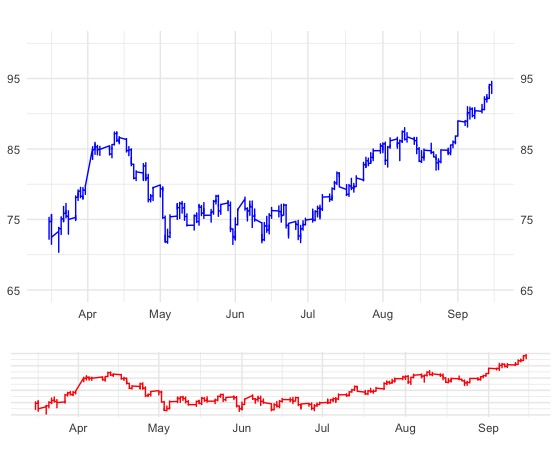
\includegraphics[width=1.0\textwidth]{Rplotbrent}
    \caption{Evoluzione del prezzo del petrolio greggio Brent generato con R (Dati forniti da Infront Italia - Borsa Italiana e Mercati Internazionali)}
    \label{fig:enter-label10}
\end{figure}


Attraverso l'utilizzo del software statistico R, è possibile impostare ed eseguire la simulazione Monte Carlo, sulla base delle indicazioni descritte precedentemente, considerando 180 rilevazioni totali, a cadenza giornaliera (contratto con valenza semestrale). In primo luogo, avendo già definito il valore del prezzo di esercizio K equivalente alla media aritmetica delle quotazioni del petrolio greggio Brent risalente all'ultimo semestre, supponendo di ritrovarci all'istante iniziale di valutazione, è possibile delineare i tre cicli di simulazione, con i quali definire il valore finale dell'opzione. Di seguito è riportato il codice utilizzato per la simulazione, con annessi risultati.


\begin{verbatim}
# Codice simulazione Monte Carlo
# Parametri dell'opzione asiatica
S0 <- 90         # Prezzo iniziale dell'attività sottostante
K <- 80.30       # Strike price
r <- 0.03        # Tasso privo di rischio
T <- 0.5         # Tempo residuo alla scadenza
sigma <- 0.25    # Volatilità
q <- 0           # Dividend yield (0 per un'opzione europea)
N <- 10000       # Numero di simulazioni Monte Carlo

MCAsianCall <- function(S0, K, T, r, sigma, N, q) {
  tau <- T / 180  # Istanti di rilevazione dei prezzi
  S <- numeric(181)
  S[1] <- S0
  m <- numeric(N)
  R <- numeric(N)
  
  for (j in 1:N) {
    for (i in 1:180) {
      epsilon <- rnorm(1)
      S[i + 1] <- S[i] * exp((r - q - (sigma^2 / 2)) * tau + 
                  sigma * sqrt(tau) * epsilon)
    }
    m[j] <- exp(1 / 181 * sum(log(S)))
    R[j] <- exp(-r * T) * mean(pmax(S[181] - K, 0))
  }
  
  MCAsianCall <- mean(R)
  return(MCAsianCall)
}
\end{verbatim}

Il valore dell'opzione asiatica simulato è: \textbf{10.93\$}. 

Dal grafico di dispersione è possibile intravedere tutti i possibili risultati generati dalle N simulazioni, dove la retta rossa indica il valore medio del payoff simulato, naturalmente non ancora attualizzato al periodo di valutazione.

\begin{figure}
     [ht]
    \centering
    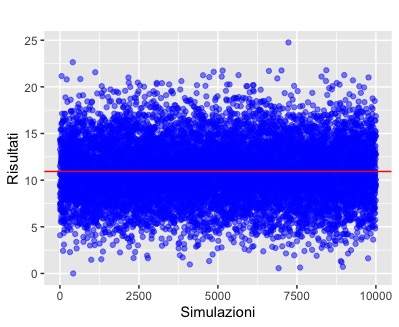
\includegraphics[width=0.7\textwidth]{Rplot03}
    \caption{Grafico di dispersione delle 10.000 simulazioni tramite R}
    \label{fig:enter-label11}
\end{figure}


Per effettuare un paragone con la metodologia introdotta nel paragrafo \textbf{4.1}, di seguito è riportato il codice per il calcolo del valore del medesimo contratto di opzione, utilizzando il modello di Vorst.


\begin{verbatim}
# Calcolo dell'Asian Option attraverso il modello di Vorst
AC <- function(sigma, S0, K, r, T, q, n) {
  tau <- T / n
  s <- 0
  
  for (i in 1:n) {
    s <- s + i
  } 
  mu_log <- log(S0) + 1/n * (r - q - (sigma^2)/2) * s * tau
  sum <- 0
  
  for (i in 1:n) {
    for (j in 1:n) {
      sum <- sum + min(i * tau, j * tau)
    }
  } 
  V <- (sigma^2) / (n^2) * sum
  somma <- 0
  
  for (i in 1:n) {
    somma <- somma + exp((r - q) * (i * tau))
  }
  
  Ea <- S0 * (somma) / (n)
  Eg <- exp(mu_log + V/2)
  Kcorr <- K - (Ea - Eg)
  d <- (mu_log - log(Y) + V) / sqrt(V)
  
  AC <- exp(-r * T) * (exp(mu_log + V/2) * pnorm(d) -
        Kcorr * pnorm(d - sqrt(V)))
  return(AC)
}
phi <- function(x) {
  pi <- 0.5 * erfc(-x / sqrt(2))
  return(pi)
}
\end{verbatim}


Il valore dell'opzione asiatica restituito dal modello è: \textbf{10.13\$}.

Come si può notare, pur essendo influenzata dall'estrazione di numeri casuali normalmente distribuiti, la simulazione Monte Carlo non si discosta di molto dal prezzo calcolato attraverso la valutazione in forma chiusa proposta dal modello di Vorst.

\section{La simulazione Monte Carlo per le opzioni Barriera}

Nel paragrafo precedente si è analizzato la serie di steps richiesti per analizzare, o meglio simulare, il possibile payoff di un'opzione esotica Asiatica. Qualora fossimo interessati ad effettuare il medesimo metodo sulle opzioni Barriera, per costituzione di quest'ultime, dovremmo porre maggiore attenzione in sede di definizione dell'algoritmo. Se, da un lato, viene omessa la prima parte di definizione e caricamento del vettore contenente le date di rilevazione del prezzo, poiché non utili ai fini della valutazione dello \textit{strike price}, dall'altro lato,il metodo Monte Carlo richiede una maggiore complessità nella definizione del ciclo interno di simulazione, dovuto alla presenza obbligatoria di regole inerenti all'attivazione o estinzione del contratto, in funzione del livello di barriera previsto. Inoltre, l'algoritmo potrebbe richiedere ulteriori regole per gestire situazioni in cui il prezzo supera o raggiunge la barriera prevista durante la simulazione. Questo potrebbe comportare un aumento della complessità dell'algoritmo e richiedere una maggiore attenzione nella sua stesura.

Tuttavia, è importante notare che l'aumento della complessità dell'algoritmo potrebbe essere bilanciato da una maggiore precisione nella simulazione dei contratti. Pertanto, è fondamentale valutare attentamente il trade-off tra complessità e accuratezza al fine di definire il ciclo interno di simulazione in modo ottimale. 


Supponiamo di voler analizzare il possibile valore di un opzione Barriera di tipo \textit{down-and-in}, dove l'holder ha il diritto di comprare o vendere l'asset sottostante ad un prezzo di esercizio K prefissato in partenza, ma con una condizione aggiuntiva. L'opzione diventa attiva e può essere esercitata solo se il prezzo dell'asset  scende al di sotto di una barriera H in un determinato momento prima della scadenza dell'opzione. In altre parole, l'opzione è "in" (attiva) se il prezzo attraversa la barriera "down" (al di sotto), altrimenti rimane "out" (non attiva).

Anche nel medesimo caso, dovremo definire tre cicli distinti, sempre annidati tra loro. Nello specifico: 
\begin{itemize}
 \item il ciclo più interno è responsabile della definizione delle finestre temporali in cui è possibile attraversare la barriera fissata. Nel caso specifico, si imposta la condizione riguardante l'attivazione della barriera (knock-in), dove è richiesto che il prezzo tocchi, a ribasso, il livello H preimpostato.


\item il ciclo intermedio considera i giorni rimanenti alla scadenza del contratto di opzione. In aggiunta, prevede l'estrazione di una serie di numeri casuali, trasformati in una sequenza $\epsilon$ normalmente distribuita, i quali verranno inseriti nella definizione dei vari livelli di prezzo generati, per ogni singolo giorno di vita del contratto. Riprendendo la formulazione precedente:

\begin{align*}
    S_{t+\uptau} = S_0 e^{(r-q-\frac{\sigma^2}{2})\uptau+\sigma\sqrt{\uptau}\epsilon}
\end{align*}

con la quale è possibile delineare la serie di prezzi richiesta per la valutazione del contratto;

\item il ciclo esterno, così come nel caso precedentemente discusso, considera sempre il numero di simulazioni N da effettuare, dove è possibile definire, successivamente, il payoff finale dell'opzione barriera:

\begin{equation}
\begin{cases}
\text{Caso call:} & C_{\textbf{BO}} = \max(S_T - K; 0) \\
\text{Caso put:} & P_{\textbf{BO}} = \max(K - S_T; 0)
\end{cases}
\end{equation}

dove:

\begin{itemize}
    \item $S_T$ = prezzo dell'opzione Barriera all'istante finale
    \item $K$ = prezzo di esercizio
\end{itemize}
\end{itemize}

In conclusione, si ripetono le varie simulazioni per N volte, utili per delineare la media dei payoff finali, in funzione della data di valutazione (considerando sempre un fattore di attualizzazione equivalente a: $e^{-r(t_n - t_0)}$)

\begin{equation}
\text{Caso call:} \quad C_{\text{OB}} = e^{-r(t_n - t_0)} \left[\frac{\sum_{i=1}^{N}\max(S_T - K, 0)}{N}\right]
\end{equation}
\begin{equation}
\text{Caso put:} \quad P_{\text{OB}} = e^{-r(t_n - t_0)} \left[\frac{\sum_{i=1}^{N}\max(K - S_T, 0)}{N}\right]
\end{equation}
\\

Anche in questo caso, supponiamo di dover valutare un opzione put \textit{down-and-in}, con il gas naturale come materia prima sottostante, a scadenza mensile con rilevazione giornaliera, con \textit{price strike} fissato a 2,50\$. Da una prima analisi preliminare condotta sui livelli di prezzo registrati nell'ultimo semestre, con rilevazione giornaliera, ricaviamo la volatilità dell'asset e l'ultimo valore registrato, che verrà utilizzato come $S_0$ nella simulazione Monte Carlo. Nello specifico:

\begin{figure}
     [ht]
    \centering
    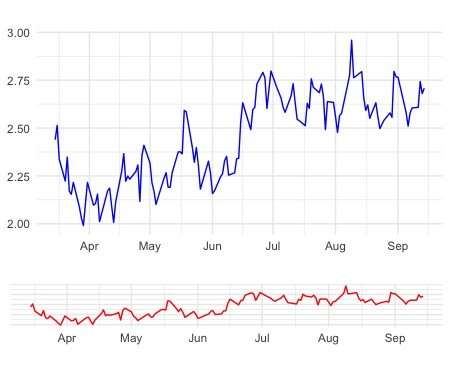
\includegraphics[width=1.0\textwidth]{Rplot04}
    \caption{Evoluzione del prezzo del gas naturale generato con R (Dati forniti da \textit{Yahoo Finance} - NY Mercantile Prezzo differito. Valuta in USD)}
    \label{fig:enter-label102}
\end{figure}

dove fissiamo $S_0$ pari a 2,70\$ come prezzo corrente dell'attività sottostante, con volatilità annua pari al 43\%.
Sulla base delle indicazioni sopra descritte, eseguendo il codice seguente in R, è possibile rilevare il payoff del contratto:

\begin{verbatim}
# Codice simulazione Monte Carlo

MCDAIP <- function(S0, K, T, r, sigma, N, q, H, n) {
  tau <- T / n
  S <- numeric(n + 1)
  S[1] <- S0
  P <- numeric(M)
  
  for (j in 1:N) {
    for (i in 1:n) {
      epsilon <- rnorm(1)
      S[i + 1] <- S[i] * exp((r - sigma * sigma - q) * tau
      + sqrt(tau) * sigma * epsilon)
    }
    
    if (min(S) > H) {
      P[j] <- max(K - S[n], 0)
    } else {
      P[j] <- 0
    }
  }
  
  MCDAIP <- exp(-r * T) * mean(P)
  return(MCDAIP)
}
\end{verbatim}

dove si pone un tasso free risk pari al 3\%, con volatilità implicita annua pari al 43\% ed un numero di rilevazioni n pari a 30. 

In funzione di questi dati, l'algoritmo genera come possibile valore finale dell'opzione put Barriera di tipo \textit{down-and-in} un payoff di 0,10\$.

Dal grafico di dispersione è possibile intravedere tutti i risultati generati dalle N simulazioni, dove la retta rossa indica il valore medio del payoff simulato.

\begin{figure}
     [ht]
    \centering
    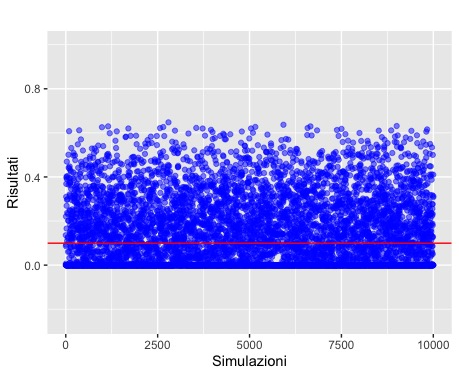
\includegraphics[width=0.7\textwidth]{Rplot24}
    \caption{Grafico di dispersione delle 10.000 simulazioni tramite R}
    \label{fig:enter-label112}
\end{figure}

Interessante è notare come questo valore si discosta dal prezzo generato attraverso l'utilizzo della metodologia proposta da Hudson, Benson, Rubinstein e Reiner. Per evidenziare le differenze, impostiamo il calcolo, sempre sul software R, utilizzando i medesimi dati:

\begin{verbatim}
# Calcolo dell'opzione put di tipo Down-And-In con il metodo Hudson, Benson,
  Rubinstein e Reiner
  
DownAndInPut <- function(sigma, S0, K, r, T, q, n, H, R) {
  S0 <- 2.70
  K <- 2.50
  H <- 2
  R <- 0.05
  r <- 0.03
  T <- 1/12
  sigma <- 0.43
  q <- 0
  n <- 30
  tau <- T/n
  eta <- r/(sigma*sigma) - 1/2
  gamma <- sqrt(eta*eta + 2*r/(sigma*sigma))
  
  a1 <- (log(S0/X)/(sigma*sqrt(T))) + (1+eta)*sigma*sqrt(T)
  a2 <- a1 - sigma*sqrt(T)
  b1 <- (log(H*H/(S0*X))/(sigma*sqrt(T))) + (1+eta)*sigma*sqrt(T)
  b2 <- b1 - sigma*sqrt(T)
  c1 <- (log(H/S0)/(sigma*sqrt(T))) + gamma*sigma*sqrt(T)
  c2 <- c1 - 2*gamma*sigma*sqrt(T)
  
  DAIOP <- (K * exp(-r * T) * phi(-a2) - S0 * phi(-a1)) +
    (K * exp(-r * T) * ((H / S0)^(2 * eta)) * phi(-b2) - 
    S0 * ((H / S0)^(2 * (eta + 1))) * phi(-b1)) +
    (R * phi(c2) - R * ((H / S0)^(eta + gamma)) * phi(c1))
 
  return(DAIOP)
}

phi <- function(x) {
  return(0.5*erfc(-x/sqrt(2)))
}
\end{verbatim}

La valutazione finale dell'opzione risulta pari a \textbf{1,39\$}. 


Confrontando il risultato ottenuto con il modello di \textit{Down-And-In} con il metodo Hudson, Benson, Rubinstein e Reiner e la simulazione Monte Carlo, si può subito notare come i due valori, non solo non coincidano, ma risultano anche essere notevolmente differenti.

Naturalmente, la simulazione Monte Carlo è solo un'approssimazione del vero comportamento del prezzo. Potrebbe accadere che, nel mondo reale, il prezzo abbia già superato la barriera, ma la simulazione non lo rileva se non la tocca effettivamente. Questa incertezza può portare a una valutazione più bassa delle opzioni "down and in" rispetto a quanto sarebbe nel caso in cui avessimo la certezza che il prezzo non abbia superato la barriera, ed è principalmente dovuta alla natura stocastica della simulazione, che cerca di approssimare il comportamento complesso dei prezzi degli asset nel tempo.

D'altra parte, le opzioni "up and out" funzionano in modo totalmente opposto. In questo caso, se il prezzo dell'asset supera una certa barriera, l'opzione si estingue. Anche qui, la simulazione Monte Carlo può sovrastimare/sottostimare il valore dell'opzione, perché potrebbe non rilevare il fatto che il prezzo dell'asset abbia superato la barriera durante l'intera simulazione.

In generale, le opzioni con la clausola "in" (come le "down and in" o le "up and in") tendono ad avere valori più bassi se valutati tramite l'algoritmo rispetto alle opzioni valutate con formule chiuse, perché c'è incertezza riguardo al superamento o al non superamento delle barriere durante la simulazione. Discorso diametralmente opposto avviene, invece, per le opzioni con clausola "out". 

Inoltre, l'incertezza può essere amplificata dalla presenza di fattori esterni che influenzano il prezzo degli asset, come eventi geopolitici o fluttuazioni economiche. Questi fattori imprevedibili possono rendere ancora più difficile la valutazione finale, aumentando l'incertezza nel processo decisionale degli investitori.

 
\section{La simulazione Monte Carlo per le opzioni Lookback}

A differenza delle Asian option e delle Barrier option, le Lookback option non richiedono una particolare attenzione in fase di definizione del codice di esecuzione dell'algoritmo Monte Carlo.

In particolare,  esse si basano esclusivamente sul prezzo massimo o minimo raggiunto dall'attività sottostante durante il periodo di validità del contratto. Questo le rende più semplici da implementare, in quanto non richiedono un monitoraggio continuo dei prezzi e la gestione di possibili livelli barriera. L'unica accortezza richiesta in fase di definizione dell'algoritmo, riguarda la scelta appropriata del periodo di validità del contratto e la corretta formulazione dei calcoli basati sul massimo o sul minimo prezzo raggiunto, in funzione della tipologia di contratto instaurata. 

Le opzioni Lookback sono quindi una scelta più efficiente in termini di risorse computazionali e possono essere facilmente incorporate nel metodo Monte Carlo senza la necessità di ulteriori complicazioni. Tuttavia, è importante considerare che questa semplicità potrebbe comportare una minore flessibilità nella gestione del rischio e dei potenziali guadagni per il trader.   

Come fase conclusiva del lavoro, è interessante poter confrontare due differenti metodologie di copertura dei rischi inerenti ad un medesimo asset sottostante.

Nello specifico, valutiamo di eseguire una simulazione Monte Carlo sul possibile payoff di una \textit{fixed Lookback option} di tipo call, che abbia come materia prima sottostante il petrolio greggio, già analizzato precedentemente nel paragrafo 5.1, e prezzo di esercizio K fisso, così da poter effettuare un confronto tra i possibili valori assunti dalle due tipologie di opzioni \textit{path dipendent}. A parità di condizioni iniziali, consideriamo quindi il seguente codice: 

\begin{verbatim}

# Codice simulazione Monte Carlo

MonteCarloFixedLookbackCall <- function(sigma, S0, r, T, q, n, N, K) {
  # Parametri
  tau <- T / n
  S <- matrix(0, n + 1, N)
  
  # Simulazione dei percorsi del prezzo del titolo
  for (j in 1:N) {
    S[1, j] <- S0
    for (i in 1:n) {
      epsilon <- rnorm(1)
      S[i + 1, j] <- S[i, j] * exp((r - sigma^2 / 2 - q) * tau + 
      sqrt(tau) * sigma * epsilon)
    }
  }
  
  # Calcolo dei payoff per ciascuna simulazione
  payoff <- numeric(N)
  for (j in 1:N) {
    max_price <- max(S[-1, j])
    payoff[j] <- max(0, max_price - K)
  }
  
  # Calcolo del valore stimato della Fixed Lookback Option Call
  MCFLC <- exp(-r * T) * mean(payoff)
   return(MCFLC)
}
\end{verbatim}

dove si pone, essendo un'opzione Fixed Lookback, il payoff è equivalente, nelle singole simulazioni, esattamente a $max_price <- max(S[-1, j])$, in cui la variabile $max_price$ rappresenta il massimo prezzo raggiunto dall'attività sottostante durante il periodo di validità del contratto. In altre parole, il valore del payoff per ciascuna simulazione è determinato esclusivamente dal massimo prezzo registrato nel percorso simulato e dalla differenza tra questo massimo prezzo e il prezzo di esercizio $K$, che invece risulta fissato in partenza.

Eseguendo l'algoritmo, l'esito finale della simulazione produce un valore pari a \textbf{22,72\$}, mentre per l'opzione Asiatica di tipo call, analizzata in precedenza, il valore prodotto era equivalente a 10,93\$. 

\begin{figure}
     [ht]
    \centering
    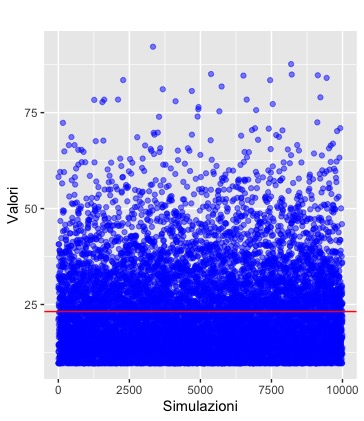
\includegraphics[width=0.5\textwidth]{Rplot08}
    \caption{Distribuzione dei Payoff della Fixed Lookback Option Call tramite R}
    \label{fig:enter-label11342}
\end{figure}


Adesso consideriamo una \textit{floating Lookback option} di tipo put, con condizioni di partenza equivalenti al caso intravisto nella valutazione dell'opzione Barriera \textit{down-and-in}. Il codice relativo alla simulazione Monte Carlo è il seguente:

\begin{verbatim}
# Codice simulazione Monte Carlo

MonteCarloELP1 <- function(sigma, S0, r, T, q, n, N) {
  S <- numeric(n + 1)
  S[1] <- S0
  tau <- T / n  # Cambio il nome da dt a tau
  
  # Simulazione del percorso del prezzo del titolo
  for (j in 1:N) {  # Cambio M in N
    for (i in 1:n) {
      epsilon <- rnorm(1)  # Cambio Y in epsilon
      S[i + 1] <- S[i] * exp((r - sigma^2 / 2 - q) * tau 
      + sqrt(tau) * sigma * epsilon)  # Cambio Y in epsilon
    }
  }
  
  # Calcolo della extrema lookback option put
  payoff <- pmax(max(S) - S[n + 1], 0)
  MCDELP <- exp(-r * T) * mean(payoff)
  
  return(MCDELP)
}
\end{verbatim}

dove si pone che il payoff deve essere maggiore di zero solo se l'opzione è \textit{in the money}, cioè se il prezzo di esercizio è maggiore del valore finale del prezzo del titolo. 

Pertanto, $pmax(max(S) - S[n + 1], 0)$ è utilizzato per assicurarsi che il payoff sia zero quando l'opzione è \textit{out of the money} (ovvero quando il prezzo di esercizio è maggiore o uguale al valore finale del prezzo del titolo).

Il risultato della simulazione è: \textbf{0.30\$}, esattamente il triplo rispetto al valore stimato nell'opzione Barriera.


\begin{figure}
     [ht]
    \centering
    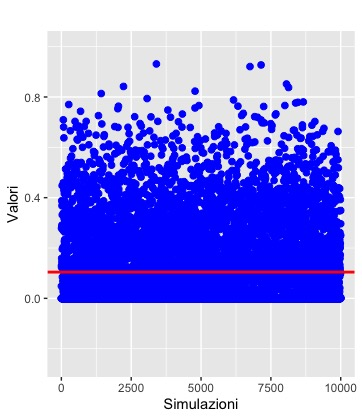
\includegraphics[width=0.5\textwidth]{Rplot05}
    \caption{Distribuzione dei Payoff della Extrema Lookback Option Put tramite R}
    \label{fig:enter-label1142}
\end{figure}

Come possiamo notare, per le opzioni Lookback, che siano standard o meno, si prospetta un valore notevolmente maggiore rispetto ad altre tipologie contrattuali, in quanto garantiscono all'holder condizioni maggiormente favorevoli, soprattutto se consideriamo l'opportunità di scegliere l'istante di esercizio direttamente a scadenza (come avviene nel primo caso), o lo strike price più conveniente (come avviene nel secondo caso.
In entrambi i casi, l'holder ha il controllo sulla decisione di esercitare l'opzione in modo da massimizzare i profitti. Questa flessibilità può comportare un costo più elevato in termini di premio dell'opzione, ma offre potenzialmente guadagni significativamente superiori.




\chapter*{Conclusione}
\addcontentsline{toc}{chapter}{Conclusione}




In questo lavoro, abbiamo esplorato in dettaglio il complesso mondo del pricing delle opzioni finanziarie e delle strategie di copertura del rischio, concentrandoci su contesti di mercato notoriamente volatili, come i mercati energetici. Il nostro percorso di ricerca è iniziato con un'attenta analisi della letteratura esistente, dalla quale abbiamo ottenuto preziose prospettive sullo stato attuale delle opzioni finanziarie e sulle sfide legate al loro prezzo.

Partendo dalle basi, abbiamo introdotto una serie di modelli matematici fondamentali, sia per la valutazione del prezzo a pronti e del prezzo a termine dell'energia elettrica, sia riguardante il valore delle opzioni analizzate. In particolare, abbiamo dedicato attenzione al modello di Vorst, strettamente collegato al celebre modello Black-Scholes, che gioca un ruolo chiave nella teoria delle opzioni asiatiche e della loro valutazione.

Ci siamo quindi addentrati nei dettagli delle Lookback option e delle Barrier option, esaminando le strategie pratiche utilizzate per gestire il rischio finanziario, con un focus specifico sul contesto aziendale, ma considerando anche aspetti di natura speculativa.

Nello specifico, abbiamo implementato concretamente un modello di valutazione per le opzioni barriera di tipo "down-and-in," utilizzando il metodo proposto da Hudson, Benson, Rubinstein e Reiner, ma applicabile, con le dovute modifiche, anche ad ulteriori sottocategorie. Nella fase successiva, abbiamo esplorato le sfide e i vincoli associati al calcolo accurato del valore di tali opzioni e dimostrato come il metodo Monte Carlo possa essere un valido strumento per stimare il loro prezzo. Abbiamo sottolineato le differenze fondamentali tra il modello di valutazione e l'approccio basato sulla simulazione casuale, evidenziando il ruolo cruciale dell'incertezza nella valutazione delle opzioni Barriera.

In seguito, ci siamo concentrati sulle opzioni "lookback," sia nella loro variante "fixed" che "floating." Abbiamo fornito un'analisi dettagliata degli algoritmi utilizzati per valutare queste opzioni, mettendo in evidenza la loro capacità di offrire maggiore flessibilità agli investitori. Tuttavia, dalle analisi abbiamo dedotto che questa variabilità può comportare costi più elevati sotto forma di premi delle opzioni, un aspetto che richiede una valutazione attenta nella fase decisionale.

In conclusione, questo studio rappresenta solamente un punto di partenza all'interno del vasto campo del pricing delle opzioni finanziarie e delle strategie di copertura. Il mondo delle opzioni è in continua evoluzione, con nuove metodologie ed approcci che vengono costantemente sviluppati e testati. Le sfide e le opportunità offerte da queste scelte finanziarie rendono la ricerca un requisito essenziale per investitori, istituzioni finanziarie e ricercatori. In particolare, i mercati energetici, con le loro caratteristiche uniche e la loro versatilità, richiedono una particolare attenzione e una ricerca continua di nuovi modelli e strumenti per una gestione sempre più efficiente.

Nel futuro, l'analisi delle opzioni finanziarie non si limiterà alla valutazione di singoli contratti, ma verrà sempre più integrata in strategie complesse di copertura e investimento. Gli operatori dei mercati energetici e finanziari dovranno continuare a perfezionare le loro conoscenze e competenze per rimanere competitivi in questo ambiente dinamico e complesso.
